\chapter{System Design and Architecture}
\label{chap:system_design}

%%%%%%%%%%%%%%%%%%%%%%%%%%%%%%%%%%%%%%%%%%%%%%%%%%%%%%
%%% SECTION 3.1 - DSR METHODOLOGY %%%
%%%%%%%%%%%%%%%%%%%%%%%%%%%%%%%%%%%%%%%%%%%%%%%%%%%%%%

\section{Research Methodology: Design Science Research (DSR)}
\label{sec:dsr_methodology}

The research presented in this thesis is constructive in nature, aimed not merely at describing or explaining a phenomenon, but at creating a novel and useful artifact to solve a real-world problem. To provide a rigorous and systematic structure for this endeavor, this study adopts the \textbf{Design Science Research (DSR)} methodology. DSR is a well-established paradigm in Information Systems research focused on the creation and evaluation of innovative IT artifacts intended to solve identified organizational problems \cite{dsr_methodology_hevner_2004}. The primary goal of DSR is to generate prescriptive design knowledge through the building and evaluation of these artifacts.

The DSR process model, as outlined by Peffers et al., provides an iterative framework that guides the research from problem identification to the communication of results \cite{dsr_methodology_peers_2006}. This thesis follows these stages, mapping them directly to its structure to ensure a logical and transparent research process:

\begin{enumerate}
    \item \textbf{Problem Identification and Motivation:} This initial stage, which involves defining the specific research problem and justifying the value of a solution, is addressed in \textbf{Chapter \ref{chap:introduction}} of this thesis. We have identified the inefficiencies of the reactive mental health support model as the core problem.

    \item \textbf{Define Objectives and Knowledge Base:} Building on the identified problem, this stage formalizes the solution objectives and anchors them in the relevant knowledge base. The initial objectives are articulated in \textbf{Chapter \ref{chap:introduction}}, and they are refined and theoretically grounded through the literature synthesis in \textbf{Chapter \ref{sec:literature_review}}.

    \item \textbf{Design and Development:} This is the core constructive phase where the artifact's architecture and functionalities are developed. This stage is the primary focus of the present chapter, \textbf{Chapter \ref{chap:system_design}}, which outlines the functional and technical blueprint of the agentic AI framework.

    \item \textbf{Demonstration:} In this stage, the designed artifact is demonstrated to solve representative instances of the problem. The functional prototype and its scenario walkthroughs are presented in \textbf{Chapter~IV}, particularly Sections \ref{sec:setup} and \ref{sec:rq1}.

    \item \textbf{Evaluation:} This stage observes and measures how well the artifact supports the solution objectives. The scenario-based tests and their analysis are reported in \textbf{Chapter~IV}, Sections \ref{sec:rq1}--\ref{sec:discussion}.

    \item \textbf{Communication of Results:} The final stage disseminates the artifact, findings, and implications to the target audience. This thesis (culminating in \textbf{Chapter~V} and supported by the appendices) serves as the primary communication vehicle.
\end{enumerate}

Stages 4-6 therefore operationalize the empirical programme for the research questions defined in Chapter \ref{sec:research_questions}. The demonstration assets in Chapter~IV (Sections~\ref{sec:setup} and \ref{sec:rq1}) instantiate the scenarios for RQ1--RQ4, while the evaluation stage reports the quantitative indicators detailed in Chapter~IV: STA sensitivity/specificity for safety (RQ1), orchestration reliability metrics such as tool-call success and latency for resilience (RQ2), rubric-based CBT quality scores for coaching (RQ3), and stability of aggregate analytics for the Insights Agent (RQ4). The communication stage synthesizes these findings in Chapter~V so that institutional stakeholders can interpret the metrics and translate them into policy and operational decisions. Together, the paragraph-level traceability between stages and metrics makes the DSR cycle a roadmap for the scenario-based evaluation that follows.

The complete workflow of this research, following the DSR methodology, is visualized in Figure \ref{fig:dsr_flowchart}. This diagram illustrates the iterative path from problem formulation through to the final conclusions and recommendations.

\definecolor{ugmBlue}{RGB}{0,73,144}
\definecolor{ugmGold}{RGB}{217,160,33}

\begin{figure}[h]
    \centering
    \resizebox{0.95\textwidth}{!}{%
    \begin{tikzpicture}[
        node distance=2.4cm,
        process/.style={rectangle, rounded corners=4pt, draw=ugmBlue, very thick, minimum width=4.0cm, minimum height=1.1cm, align=center, fill=ugmBlue!6},
        arrow/.style={-Latex, thick, ugmBlue},
        looparrow/.style={-Latex, thick, ugmGold}
    ]
        \node[process] (problem) {Problem Identification\\\footnotesize (Chapter~\ref{chap:introduction})};
        \node[process, right=of problem] (literature) {Objectives \& Knowledge Base\\\footnotesize (Ch.~\ref{chap:introduction},~\ref{sec:literature_review})};
        \node[process, right=of literature] (design) {Artifact Design \& Development\\\footnotesize (Chapter~\ref{chap:system_design})};
        \node[process, right=of design] (implementation) {Prototype Demonstration\\\footnotesize (Chapter~IV, Sec.~\ref{sec:setup})};
        \node[process, right=of implementation] (evaluation) {Scenario Evaluation\\\footnotesize (Chapter~IV, Secs.~\ref{sec:rq1}--\ref{sec:discussion})};
        \node[process, right=of evaluation] (conclusion) {Communication of Results\\\footnotesize (Chapter~V)};

        \draw[arrow] (problem) -- (literature);
        \draw[arrow] (literature) -- (design);
        \draw[arrow] (design) -- (implementation);
        \draw[arrow] (implementation) -- (evaluation);
        \draw[arrow] (evaluation) -- (conclusion);
        \draw[looparrow, looseness=1.1] (evaluation.south) to[out=-90, in=-90] (design.south);
        \draw[looparrow, looseness=1.2] (implementation.north) to[out=90, in=90] (literature.north);
    \end{tikzpicture}}
    \caption{The Design Science Research (DSR) process model as applied in this thesis. Iterative loops capture how evaluation informs redesign and how implementation insights update the knowledge base.}
    \label{fig:dsr_flowchart}
\end{figure}

%%%%%%%%%%%%%%%%%%%%%%%%%%%%%%%%%%%%%%%%%%%%%%%%%%%%%%%
%%% SECTION 3.2 - SYSTEM OVERVIEW %%%
%%%%%%%%%%%%%%%%%%%%%%%%%%%%%%%%%%%%%%%%%%%%%%%%%%%%%%%

\section{System Overview and Conceptual Design}

The artifact proposed and developed in this research is a novel agentic AI framework designed to address the systemic inefficiencies of traditional, reactive mental health support models in Higher Education Institutions. The conceptual architecture is predicated on the principles of a Multi-Agent System (MAS), wherein a suite of collaborative, specialized intelligent agents, collectively termed the \textbf{Safety Agent Suite}, work in concert to create a proactive, scalable, and data-driven support ecosystem. This framework is designed not as a monolithic application, but as a dynamic, closed-loop system that operates on two interconnected levels: a micro-level loop for real-time, individual student support and a macro-level loop for strategic, institutional oversight and proactive intervention \cite{kashiv2025aidrivennetworks, nwoke2025insightautomation}.

The system's primary entities and their designated interaction points are illustrated in the conceptual context diagram in Figure \ref{fig:context_diagram}. These entities are:
\begin{itemize}
    \item \textbf{Students:} As the primary users, students interact with the system's conversational interface (UGM-AICare's `/aika` page). This serves as their direct entry point to the support ecosystem, where they engage with the agents responsible for coaching and immediate assistance.
    \item \textbf{University Staff/Counselors:} As the system's administrators and clinical supervisors, these stakeholders interact with a secure Admin Dashboard. This interface serves as the human-in-the-loop control center, providing aggregated analytics for strategic decision-making and a case management system for handling high-risk escalations.
    \item \textbf{The Agentic AI Backend:} This is the core computational engine of the framework. It hosts the four agents of the Safety Agent Suite, manages their stateful interactions via LangGraph, and serves as the central hub for all data processing, logic execution, and communication with external services and databases.
\end{itemize}

\begin{table}[h]
    \centering
    \caption{Comparison of representative university well-being platforms.}
    \label{tab:wellbeing_comparison}
    \begin{tabular}{p{3.4cm}p{3.6cm}p{3.6cm}p{3.6cm}}
        \toprule
        \textbf{Platform} & \textbf{Primary Modality} & \textbf{Safety/Privacy Posture} & \textbf{Contrast with Safety Agent Suite} \\
        \midrule
        Woebot Campus Programme\cite{FIND_CITATION_PLACEHOLDER} & Daily CBT-aligned chatbot sessions with journaling prompts. & Crisis disclaimers and human referral prompts, but escalation remains manual and analytics are limited. & Lacks dedicated triage agent or orchestration guardrails; actionable insights are not automated, restricting proactive interventions. \\
        Togetherall Peer Community\cite{FIND_CITATION_PLACEHOLDER} & Moderated peer-to-peer forums with clinician oversight and resource hubs. & Strong anonymity policies and moderator workflows, yet response time depends on human moderators. & Provides community support but no automated coaching, triage, or strategic analytics loop as offered by the Safety Agent Suite. \\
        Kognito ``At-Risk'' Simulations\cite{FIND_CITATION_PLACEHOLDER} & Scenario-based training to help faculty/students identify and refer distressed peers. & Focuses on awareness; no live data capture or privacy-sensitive storage since it is a training tool. & Educates stakeholders but does not deliver operational support, automated escalation, or continuous monitoring of student well-being. \\
        \bottomrule
    \end{tabular}
\end{table}

Conceptually, the framework's architecture is best understood as two distinct but integrated operational loops:

\begin{enumerate}
    \item \textbf{The Real-Time Interaction Loop:} This loop handles immediate, synchronous interactions with individual students. When a student sends a message, it is first processed by the \textbf{Safety Triage Agent (STA)} for risk assessment. If the context is deemed safe, the \textbf{Support Coach Agent (SCA)} takes over to provide personalized, evidence-based guidance. Should the user require administrative assistance, such as scheduling an appointment, the workflow is seamlessly handed off to the \textbf{Service Desk Agent (SDA)}. This loop is designed for high-availability, low-latency responses, ensuring that students receive immediate and appropriate support.
    \item \textbf{The Strategic Oversight Loop:} This loop operates on a longer, asynchronous timescale to enable proactive, institution-wide strategy. The \textbf{Insights Agent (IA)} periodically analyzes the anonymized, aggregated data from all student interactions. It generates reports on population-level well-being trends, sentiment analysis, and emerging topics of concern. These reports are delivered to administrators via the Admin Dashboard, providing the empirical evidence needed for data-driven resource allocation, such as commissioning new workshops or adjusting counseling staff schedules. This loop directly addresses the "insight-to-action" gap that plagues current systems \cite{nwoke2025insightautomation, jorno2018actionableinsight}.
\end{enumerate}

The synergy between these two loops is the cornerstone of the framework's design. The real-time loop gathers the data that fuels the strategic loop, while the insights from the strategic loop can be used to configure and improve the proactive interventions delivered by the real-time loop, creating a continuously learning and adaptive support ecosystem.

\subsubsection{Orchestration Alternatives and Rationale}

Classical multi-agent systems literature distinguishes between centralized planners, market-based negotiation schemes, and more recent graph-structured controllers for coordinating autonomous agents \cite{wooldridge1995intelligentagents,wooldridge2009introductionmas}. Contemporary surveys focused on LLM-powered agents show that orchestration frameworks such as LangGraph provide deterministic state persistence, guardrails, and cycle control that are difficult to obtain in purely contract-net or ad-hoc workflow engines \cite{yang2025aiagentprotocols,tran2025multiagentcollaboration,yu2025agentworkflow}. Table~\ref{tab:orchestration_patterns} contrasts these patterns and summarizes why the Safety Agent Suite adopts a graph-based orchestration.

\begin{table}[h]
    \centering
    \caption{Comparison of orchestration patterns for the Safety Agent Suite.}
    \label{tab:orchestration_patterns}
    \begin{tabular}{p{3.4cm}p{4.0cm}p{4.0cm}}
        \toprule
        \textbf{Approach} & \textbf{Coordination Strengths} & \textbf{Limitations and Implications for Safety Agent Suite} \\
        \midrule
        Centralized workflow/planner \cite{wooldridge2009introductionmas} & Deterministic control flow and straightforward verification of simple pipelines. & Brittle when the conversation requires branching or repeated loops; a single orchestrator becomes a failure hotspot and hinders human-in-the-loop escalations needed for STA. \\
        Contract-net / market-based negotiation \cite{wooldridge1995intelligentagents,tran2025multiagentcollaboration} & Decentralized task allocation and flexibility for loosely coupled agents. & Negotiation latency and probabilistic assignment make it difficult to guarantee triage deadlines and safety invariants; insufficient for crisis escalation SLAs. \\
        Graph-based, stateful orchestrator (LangGraph) \cite{yang2025aiagentprotocols,yu2025agentworkflow} & Explicit state persistence, guard conditions, and cyclic workflows that support guardrails, retries, and logging. & Requires deliberate state-schema design and emerging tooling, but best aligns with the need for deterministic escalation paths, auditing, and metric capture in Chapters~IV and~V. \\
        \bottomrule
    \end{tabular}
\end{table}

In practice, LangGraph's stateful edges allow the Safety Triage Agent to enforce risk-score thresholds before delegating to the Support Coach Agent, while still preserving the ability to retry, log, and escalate without bespoke infrastructure. This orchestration choice therefore underpins the evaluation metrics reported later for tool-call reliability, latency, and auditability.

\begin{figure}[h]
    \centering
    \resizebox{0.95\textwidth}{!}{%
    \begin{tikzpicture}[
        entity/.style={rectangle, rounded corners=4pt, draw=ugmBlue, very thick, fill=ugmBlue!6, align=center, minimum width=3.6cm, minimum height=1.4cm},
        external/.style={entity, fill=white},
        datastore/.style={rectangle, draw=ugmBlue, thick, fill=ugmBlue!10, align=center, minimum width=4.4cm, minimum height=1.2cm},
        innerbox/.style={rectangle, rounded corners=3pt, draw=ugmBlue!70, fill=ugmBlue!12, minimum width=3.0cm, minimum height=0.85cm, font=\footnotesize, align=center},
        arrow/.style={-Latex, thick, ugmBlue},
        dashedarrow/.style={-Latex, thick, ugmBlue, dashed}
    ]
        \node[external] (student) {Student\\\footnotesize UGM-AICare App};
        \node[entity, right=3.8cm of student, minimum width=4.6cm, minimum height=4.5cm] (backend) {};
        \node at (backend.north) [yshift=-0.35cm, font=\bfseries\small, text=ugmBlue] {Safety Agent Suite};
        \node[innerbox] (sta) at ([yshift=0.75cm]backend.center) {Safety Triage Agent};
        \node[innerbox, below=0.2cm of sta] (sca) {Support Coach Agent};
        \node[innerbox, below=0.2cm of sca] (sda) {Service Desk Agent};
        \node[innerbox, below=0.2cm of sda] (ia) {Insights Agent};
        \node[external, right=3.6cm of backend] (staff) {University Staff\\\footnotesize Admin Dashboard};
        \node[datastore, below=1.8cm of backend] (dataplatform) {Data Platform\\\footnotesize Encrypted storage \& analytics};
        \node[external, above=1.8cm of backend] (llm) {LLM Service\\\footnotesize (Gemini API)};

        \draw[arrow] (student) -- node[above, font=\footnotesize]{Messages, mood signal} (backend);
        \draw[arrow] (backend) -- node[above, font=\footnotesize]{Coach responses, resources} (student);
        \draw[arrow] (backend) -- node[above, font=\footnotesize]{Alerts, insights} (staff);
        \draw[dashedarrow] (staff) -- node[below, font=\footnotesize]{Escalation reviews, configuration} (backend);
        \draw[arrow] (backend) -- node[right, font=\footnotesize]{Anonymised logs, metrics} (dataplatform);
        \draw[dashedarrow] (dataplatform) -- node[left, font=\footnotesize]{Aggregated reports} (backend);
        \draw[arrow] (backend) -- node[right, font=\footnotesize]{Structured prompts, tool calls} (llm);
        \draw[dashedarrow] (llm) -- node[left, font=\footnotesize]{Generated responses} (backend);
    \end{tikzpicture}}
    \caption{High-level context of the Safety Agent Suite showing primary stakeholders, orchestration boundaries, and data exchanges. Dashed arrows denote supervisory or configuration interactions.}
    \label{fig:context_diagram}
\end{figure}

%%%%%%%%%%%%%%%%%%%%%%%%%%%%%%%%%%%%%%%%%%%%%%%%%%%%%%%
%%% SECTION 3.3 - FUNCTIONAL ARCHITECTURE %%%
%%%%%%%%%%%%%%%%%%%%%%%%%%%%%%%%%%%%%%%%%%%%%%%%%%%%%%%

\section{Functional Architecture: The Agentic Core}
\label{chap:functional_architecture}

The functional architecture of the framework is designed as a Multi-Agent System (MAS), where the system's overall intelligence and capability emerge from the coordinated actions of its four specialized agents. This section details the "what" of the system by defining the specific role, operational logic, and capabilities of each agent within the \textbf{Safety Agent Suite}. Each agent functions as a distinct component within the LangGraph state machine, perceiving its environment through the shared state, executing its logic, and updating the state with its results.

\subsection{The Safety Triage Agent (STA): The Real-Time Guardian}

\subsubsection{Goal}
The primary objective of the STA is to function as a real-time, automated safety monitor for every user interaction. Its goal is to assess the immediate risk level of a user's conversation to detect potential crises and trigger an appropriate escalation protocol without delay, ensuring that safety is the foremost priority of the system.

\subsubsection{Perception (Inputs)}
The STA perceives the conversational environment by intercepting each user message before it is processed by other agents. Its primary input is the raw text of the user's current utterance. Let $M_t$ be the user's message at time $t$. The STA's perception is solely focused on this message:
\begin{itemize}
    \item \textbf{Current User Message ($M_t$):} A string containing the user's latest input.
\end{itemize}

\subsubsection{Processing Logic}
The core logic of the STA is a high-speed classification task. Upon receiving the message $M_t$, the agent invokes a specialized function, powered by the Gemini 2.5 Pro model, to classify the message into one of several predefined risk categories. The classification function, $f_{STA}$, can be represented as:
$$ R_t = f_{STA}(M_t; \theta_{LLM}) $$
where $\theta_{LLM}$ represents the parameters of the underlying Large Language Model, and the output, $R_t$, is an element of the set of possible risk levels, $R \in \{\text{Low, Moderate, Critical}\}$. The prompt for this classification is highly optimized for speed and accuracy, instructing the model to evaluate the text for indicators of self-harm, severe distress, or explicit requests for urgent help.

\subsubsection{Action (Outputs)}
Based on the classification result $R_t$, the STA's action is to update the system's state, which in turn determines the next step in the LangGraph workflow.
\begin{itemize}
    \item \textbf{State Update:} The agent's primary output is an update to the shared state graph, setting the \texttt{risk\_level} variable to the value of $R_t$.
    \item \textbf{Trigger Escalation (if $R_t$ = Critical):} If a critical risk is detected, the agent's action triggers a conditional edge in the graph that invokes the \texttt{escalate\_crisis} tool. This tool flags the conversation on the Admin Dashboard, logs the event, and instructs the Service Desk Agent (SDA) to create a high-priority case. It also immediately presents the user with pre-defined emergency resources.
\end{itemize}

\begin{itemize}
    \item \textbf{Design Rationale:} Assumes each incoming $M_t$ is UTF-8 text already filtered for profanity/noise; applies a calibrated confidence threshold (LLM softmax score $\geq0.6$) before labelling critical risk, otherwise defers to a human counselor; prompt template and \texttt{escalate\_crisis} schema were validated on the synthetic crisis corpus and scenario metrics reported in Chapter~\ref{sec:rq1}.\cite{FIND_CITATION_PLACEHOLDER}
\end{itemize}

\subsection{The Support Coach Agent (SCA): The Empathetic Mentor}

\subsubsection{Goal}
The SCA is the primary user-facing conversational agent, designed to provide personalized, evidence-based mental health coaching. Its goal is to engage the student in a supportive, empathetic dialogue, guiding them through structured self-help modules based on established therapeutic principles like Cognitive Behavioral Therapy (CBT), and to sustain engagement through gentle progress tracking and timely check-ins.

\subsubsection{Perception (Inputs)}
The SCA operates on the history of the conversation and the user's profile. Its key inputs from the state graph are:
\begin{itemize}
    \item \textbf{Conversation History ($H_{t-1}$):} The full transcript of the conversation up to the previous turn.
    \item \textbf{User's Current Message ($M_t$):} The message deemed safe by the STA.
    \item \textbf{User State:} Information about the user's progress, including completed modules and outstanding check-ins.
\end{itemize}

\subsubsection{Processing Logic}
The SCA's logic is generative and context-aware. It uses the Gemini 2.5 Pro model to generate a conversational response, $A_t$, that is empathetic and relevant to the user's message and history.
$$ A_t = f_{SCA}(M_t, H_{t-1}; \theta_{LLM}) $$
This agent has access to a toolset that allows it to retrieve and present structured content. When a user's query or the conversation flow indicates a need for a specific skill (e.g., managing anxiety), the SCA can decide to invoke its \texttt{retrieve\_cbt\_module} tool to fetch and present the relevant exercise.

\subsubsection{Action (Outputs)}
\begin{itemize}
    \item \textbf{Conversational Response:} A human-like text response to be displayed to the user.
    \item \textbf{Tool Call (Content Delivery):} Invocation of tools to present CBT exercises or other self-help modules.
    \item \textbf{Tool Call (Progress Logging):} Upon completion of a module, the SCA can call the \texttt{record\_module\_completion} tool to update the student's progress log in the shared state and database.
\end{itemize}

\begin{itemize}
    \item \textbf{Design Rationale:} Assumes the STA has sanitised $M_t$ and that $H_{t-1}$ retains fewer than 50 dialogue turns to bound context length; enforces refusal policies for out-of-scope clinical topics and escalates administrative intents to the SDA; prompts and tool schemas were peer-reviewed with counselling staff and evaluated via the rubric-based assessment in Chapter~\ref{sec:rq2}.\cite{FIND_CITATION_PLACEHOLDER}
\end{itemize}

\subsection{The Service Desk Agent (SDA): The Administrative Orchestrator}

\subsubsection{Goal}
The SDA functions as the administrative backbone of the support system. Its primary goal is to automate the operational workflows related to clinical case management and resource scheduling, thereby reducing the manual burden on university staff and ensuring that escalations and requests are handled efficiently and reliably.

\subsubsection{Perception (Inputs)}
The SDA is primarily triggered by events from other agents or direct commands from the Admin Dashboard. Its inputs are structured data, not conversational text:
\begin{itemize}
    \item \textbf{Escalation Event:} A signal from the STA containing the conversation ID and risk level of a flagged case.
    \item \textbf{Scheduling Request:} A structured request from the SCA (initiated by a user) containing the user's ID and desired appointment times.
    \item \textbf{Admin Commands:} Directives from a human administrator via the dashboard (e.g., "close case," "add note").
\end{itemize}

\subsubsection{Processing Logic}
The SDA's logic is procedural and tool-based. It does not engage in open-ended conversation but rather executes a sequence of pre-defined actions based on its inputs. For example, upon receiving an escalation event, its logic is to execute the \texttt{create\_case} tool, followed by the \texttt{assign\_case\_status} tool with the "New" parameter.

\subsubsection{Action (Outputs)}
\begin{itemize}
    \item \textbf{Database Operations:} The SDA's primary actions are database mutations, such as creating, updating, or closing case records in the clinical management database.
    \item \textbf{API Calls to External Services:} It can interact with external calendar systems to check for counselor availability and book appointments.
    \item \textbf{Notifications:} It sends automated email or dashboard notifications to counselors when a new case is assigned to them or when a student books an appointment.
\end{itemize}

\begin{itemize}
    \item \textbf{Design Rationale:} Assumes structured events carry validated UUIDs, ISO-8601 timestamps, and pass schema validation upstream; enforces idempotent tool execution with exponential backoff and escalates to human staff after three failed retries; tool schemas were exercised in integration tests summarised in Chapter~\ref{sec:rq2}.\cite{FIND_CITATION_PLACEHOLDER}
\end{itemize}

\subsection{The Insights Agent (IA): The Strategic Analyst}

\subsubsection{Goal}
The IA is designed to function as the institution's automated well-being analyst. Its goal is to autonomously process anonymized, aggregated conversation data to identify population-level mental health trends, sentiment shifts, and emerging topics of concern. This provides the institution with actionable, data-driven intelligence to inform resource allocation and proactive strategy.

\subsubsection{Perception (Inputs)}
The IA is activated by a time-based trigger (e.g., a weekly Cron job) and its primary input is the entire corpus of anonymized conversation logs.
\begin{itemize}
    \item \textbf{Time-Based Trigger:} A signal from the APScheduler to begin its analysis.
    \item \textbf{Anonymized Database Access:} Read-only access to the \texttt{conversation\_logs} table, from which all personally identifiable information (PII) has been redacted.
\end{itemize}

\subsubsection{Processing Logic}
The IA's logic involves a pipeline of Natural Language Processing (NLP) tasks performed on the collected data. This includes:
\begin{itemize}
    \item \textbf{Topic Modeling:} Using algorithms like Latent Dirichlet Allocation (LDA) or modern transformer-based clustering to identify the most prevalent topics of discussion (e.g., "exam stress," "social isolation").
    \item \textbf{Sentiment Analysis:} Calculating the overall sentiment score for the student population over the given period and tracking its change over time.
    \item \textbf{Summarization:} Using the Gemini 2.5 Pro model to generate concise, human-readable summaries of the key findings from the topic and sentiment analysis.
\end{itemize}

\subsubsection{Action (Outputs)}
\begin{itemize}
    \item \textbf{Structured Report Generation:} The final output is a structured report (e.g., in JSON or PDF format) containing visualizations (e.g., charts of topic frequency over time) and the generated summaries.
    \item \textbf{Dashboard Update:} The agent pushes this report to the Admin Dashboard, updating the analytics view for university staff.
    \item \textbf{Email Notification:} It can be configured to automatically email the report to a list of stakeholders, such as the head of counseling services.
\end{itemize}

\begin{itemize}
    \item \textbf{Design Rationale:} Assumes access to anonymised logs aggregated with $k\geq50$ users and retained for no longer than 90 days; enforces differential privacy noise addition (placeholder $\epsilon=1.0$) and suppresses outputs below the threshold; analytical prompts and pipelines were stress-tested via the stability checks in Chapter~\ref{sec:rq4}.\cite{FIND_CITATION_PLACEHOLDER}
\end{itemize}

\begin{figure}[h]
    \centering
    \resizebox{0.95\textwidth}{!}{%
    \begin{tikzpicture}[
        node distance=2.3cm,
        actor/.style={rectangle, rounded corners=4pt, draw=ugmBlue, very thick, fill=white, align=center, minimum width=2.8cm, minimum height=1.1cm},
        agent/.style={rectangle, rounded corners=4pt, draw=ugmBlue, thick, fill=ugmBlue!7, align=center, minimum width=3.0cm, minimum height=1.1cm, font=\footnotesize},
        datastore/.style={rectangle, draw=ugmBlue, thick, fill=ugmBlue!10, align=center, minimum width=3.0cm, minimum height=1.1cm, font=\footnotesize},
        arrow/.style={-Latex, thick, ugmBlue},
        dashedarrow/.style={-Latex, thick, ugmBlue, dashed}
    ]
        \node[actor] (user) {Student};
        \node[agent, right=of user] (sta) {Safety Triage Agent};
        \node[agent, right=of sta] (sca) {Support Coach Agent};
        \node[actor, right=of sca] (studentReturn) {Student Response};

        \draw[arrow] (user) -- node[above, font=\footnotesize]{Message} (sta);
        \draw[arrow] (sta) -- node[above, font=\footnotesize]{Safe prompt} (sca);
        \draw[arrow] (sca) -- node[above, font=\footnotesize]{Coaching reply} (studentReturn);

        \node[agent, below=2.0cm of sta] (sda) {Service Desk Agent};
        \node[actor, right=of sda] (admin) {Counselor / Staff};
        \draw[arrow] (sta) -- node[left, font=\footnotesize]{Escalation} (sda);
        \draw[arrow] (sda) -- node[above, font=\footnotesize]{Case alert} (admin);
        \draw[dashedarrow] (admin) -- node[below, font=\footnotesize]{Resolution update} (sda);

        \node[datastore, below=2.0cm of sca] (progress) {Progress Logs};
        \draw[arrow] (sca) -- node[right, font=\footnotesize]{Module completion} (progress);

        \node[agent, below=1.6cm of progress] (ia) {Insights Agent};
        \node[datastore, right=of ia] (analytics) {Aggregated Reports};
        \draw[arrow] (progress) -- node[right, font=\footnotesize]{Anonymised traces} (ia);
        \draw[arrow] (ia) -- node[above, font=\footnotesize]{Weekly summary} (analytics);
        \draw[arrow] (ia) -- node[left, font=\footnotesize]{Trend alert} (admin);
    \end{tikzpicture}}
    \caption{Data flow between the Safety Agent Suite and its users. Solid arrows show operational data paths; dashed arrows show supervisory feedback.}
    \label{fig:dfd}
\end{figure}


\section{Security and Privacy Threat Model}
\label{sec:threat_model}

Protecting student data and maintaining institutional trust require an explicit articulation of adversaries, assets, and mitigations. Table~\ref{tab:threat_model} summarises the threat model adopted for the Safety Agent Suite, drawing on STRIDE/LINDDUN heuristics and privacy-by-design obligations.\cite{FIND_CITATION_PLACEHOLDER}

\begin{table}[h]
    \centering
    \caption{Threat model overview.}
    \label{tab:threat_model}
    \begin{tabular}{p{3.0cm}p{3.5cm}p{3.5cm}p{3.5cm}}
        \toprule
        \textbf{Actor / Threat} & \textbf{Targeted Asset} & \textbf{Likely Impact} & \textbf{Mitigations / Controls} \\
        \midrule
        Compromised student account & Conversation logs, risk flags & Exposure of sensitive disclosures; spoofed escalations & MFA and device attestation (frontend); STA confidence thresholds with human verification; audit trail review (Chapter~\ref{sec:rq1}). \\
        Malicious insider (staff) & Case notes, progress logs & Unauthorised browsing or data exfiltration & Role-based access control, immutable audit logs, case access alerts, quarterly review. \\
        External attacker (API abuse) & Backend endpoints, tooling & Prompt injection, denial of service, data tampering & API gateway with rate limiting, input sanitation, LangGraph guardrails, automated anomaly detection on latency/tool-failure metrics. \\
        Analytics linkage attack & Aggregated insights & Re-identification through small cohorts & Minimum cohort size $k\geq50$, differential privacy noise (placeholder $\epsilon=1.0$), suppression of rare categories (Chapter~\ref{sec:rq4}). \\
        Model supply-chain risks & LLM outputs / prompts & Hallucinated or unsafe responses & Structured prompts, refusal and escalation policies, prompt/response logging with red-team testing cadence. \\
        Infrastructure failure & Agent orchestration state & Service outage, message loss & Stateless frontend, checkpointed LangGraph state, automated failover for database replicas, latency SLOs monitored (Section~\ref{chap:technical_architecture}). \\
        \bottomrule
    \end{tabular}
\end{table}

These mitigations align with institutional policies and inform the evaluation metrics in Chapter~IV (e.g., STA sensitivity to avoid under- or over-escalation) and the privacy discussion in Chapter~V. Residual risks---such as novel jailbreak prompts or emergent privacy attacks---are addressed through scheduled red-team exercises, update audits for commercial APIs, and continuous monitoring of anomaly indicators.


%%%%%%%%%%%%%%%%%%%%%%%%%%%%%%%%%%%%%%%%%%%%%%%%%%%%%%%
%%% SECTION 3.4 - TECHNICAL ARCHITECTURE %%%
%%%%%%%%%%%%%%%%%%%%%%%%%%%%%%%%%%%%%%%%%%%%%%%%%%%%%%%

\section{Technical Architecture}
\label{chap:technical_architecture}

This section details the "how" of the system, providing the engineering blueprint for the agentic AI framework. The architecture is designed following a modern, service-oriented pattern, which decouples the primary components of the system into distinct, independently deployable services. This approach enhances maintainability, scalability, and promotes a clean separation of concerns \cite{newman2021buildingmicroservices, richards2020softwarearchitecture}. The framework consists of three core services: a unified frontend application, a backend service that houses the agentic core, and a data persistence service for all storage needs.

\subsection{Overall System Architecture}
\label{sec:overall_system_architecture}

The overall technical architecture is visualized in Figure \ref{fig:system_architecture_diagram}. It is a monolithic frontend-backend structure composed of three primary services that work in concert to deliver the full functionality of the framework to both students and administrators.

\begin{enumerate}
    \item \textbf{Frontend Service (UGM-AICare Web Application):} This is a comprehensive web application built using the \textbf{Next.js} framework. It serves two distinct user-facing roles from a single codebase:
        \begin{itemize}
            \item \textbf{The User Portal:} This is the interface for students. It provides access to features such as a journaling system, a user dashboard for tracking progress, and the `/aika` chat interface for direct interaction with the Support Coach Agent (SCA) and Safety Triage Agent (STA). It also handles features like appointment scheduling with counselors.
            \item \textbf{The Admin Dashboard:} This is a secure, role-protected area of the application for university staff and counselors. Its responsibilities include rendering the analytics and insights provided by the Insights Agent (IA), displaying real-time alerts for flagged conversations, and providing a case management system to act on escalations from the STA and SDA.
        \end{itemize}
    \item \textbf{Backend Service (The Agentic Core):} This service is the "brain" of the entire operation, built using the \textbf{FastAPI} Python framework. It exposes a \textbf{REST API} through which the unified Next.js frontend communicates. The backend is responsible for handling all business logic, including processing incoming chat messages from the User Portal, orchestrating the agents within the LangGraph state machine, making calls to the Google Gemini API, and interacting with the database. The asynchronous capabilities of FastAPI are critical for efficiently managing multiple concurrent conversations and long-running agentic tasks.
    \item \textbf{Data Persistence Service:} A \textbf{PostgreSQL} relational database serves as the single source of truth for the system. It is responsible for storing all persistent data, including user information (anonymized), conversation logs, clinical case data, and generated reports.
\end{enumerate}

\subsubsection{Capacity Planning and Performance Targets}

To ensure the architecture meets the safety and responsiveness requirements evaluated in Chapter~\ref{sec:rq1}, we define the following planning assumptions:
\begin{itemize}
    \item \textbf{Latency budgets:} STA classification must complete within 250~ms p95 and 500~ms p99, while end-to-end conversational responses (STA~+~SCA) target 1.5~s p95 under nominal load. Scenario results in Chapter~\ref{sec:rq1} and Chapter~\ref{sec:rq2} will be benchmarked against these SLOs.
    \item \textbf{Concurrency expectations:} The system is sized for 500 concurrent student sessions (peak exam season) with headroom to burst to 1,000. Each FastAPI worker handles approximately 20 concurrent conversations; horizontal scaling of backend pods maintains SLA compliance.
    \item \textbf{Horizontal scaling strategy:} Stateless Next.js frontend instances auto-scale behind a CDN; the FastAPI+LangGraph service scales via container orchestration (e.g., Kubernetes HPA) using CPU and latency metrics; PostgreSQL employs read replicas for analytics workloads while the primary instance handles transactional writes. Queueing (e.g., Redis streams) buffers asynchronous Insights Agent jobs to decouple heavy analytics from real-time triage.
    \item \textbf{Resilience and monitoring:} Service-level indicators (SLIs) include STA false-negative rate, tool-call success percentage, queue depth, and database replication lag. Alert thresholds align with risk tolerances captured in the threat model (Table~\ref{tab:threat_model}).\cite{FIND_CITATION_PLACEHOLDER}
\end{itemize}

Communication between the unified frontend and the backend is exclusively handled via a secure, stateless REST API. The backend service is the only component with direct access to the database, ensuring a clear and secure data access pattern. This architecture allows for a cohesive user experience while maintaining a strong separation between presentation logic (frontend) and business logic (backend).

\begin{figure}[h]
    \centering
    \begin{tikzpicture}[
        box/.style={rectangle, draw=ugmBlue, very thick, rounded corners=6pt, align=center, fill=ugmBlue!5},
        subbox/.style={rectangle, draw=ugmBlue!70, thick, rounded corners=4pt, align=center, fill=white, minimum width=3.3cm, minimum height=1.1cm, font=\footnotesize},
        actor/.style={rectangle, draw=ugmBlue, very thick, rounded corners=4pt, fill=white, align=center, minimum width=2.7cm, minimum height=1.1cm},
        datastore/.style={rectangle, draw=ugmBlue, thick, align=center, fill=ugmBlue!10, minimum width=3.7cm, minimum height=1.2cm},
        arrow/.style={-Latex, thick, ugmBlue},
        doublearrow/.style={<->, >=Latex, thick, ugmBlue}
    ]
        \node[actor] (student) {Student};
        \node[box, right=2.2cm of student, minimum width=5.6cm, minimum height=4.8cm] (frontend) {};
        \node at (frontend.north) [yshift=-0.35cm, font=\bfseries\small, text=ugmBlue] {Frontend Service (Next.js)};
        \node[subbox] (portal) at ([yshift=0.9cm]frontend.center) {User Portal / `/aika` Chat};
        \node[subbox, below=0.4cm of portal] (dashboard) {Admin Dashboard};
        \node[subbox, below=0.4cm of dashboard, minimum width=3.3cm] (shared) {Shared UI Components};

        \node[box, right=3.0cm of frontend, minimum width=6.0cm, minimum height=5.4cm] (backend) {};
        \node at (backend.north) [yshift=-0.35cm, font=\bfseries\small, text=ugmBlue] {Backend Service (FastAPI)};
        \node[subbox, minimum width=4.2cm] (core) at ([yshift=1.1cm]backend.center) {Agentic Core (LangGraph)};
        \node[subbox, below=0.35cm of core, minimum width=4.2cm] (sta) {Safety Triage Agent};
        \node[subbox, below=0.25cm of sta, minimum width=4.2cm] (sca) {Support Coach Agent};
        \node[subbox, below=0.25cm of sca, minimum width=4.2cm] (sda) {Service Desk Agent};
        \node[subbox, below=0.25cm of sda, minimum width=4.2cm] (ia) {Insights Agent};

        \node[datastore, below=2.5cm of backend] (database) {Database Service (PostgreSQL)};
        \node[actor, right=2.6cm of backend] (gemini) {Google Gemini API};
        \node[actor, above=2.6cm of frontend] (admin) {Counselor / Staff};

        \draw[doublearrow] (frontend) -- node[above, font=\footnotesize]{REST API (HTTPS)} (backend);
        \draw[arrow] (backend) -- node[right, font=\footnotesize]{Direct DB connection} (database);
        \draw[arrow] (backend) -- node[above, font=\footnotesize]{Structured prompts \& tool calls} (gemini);
        \draw[arrow] (student) -- node[above, font=\footnotesize]{Web / Mobile access} (portal.west);
        \draw[arrow] (admin) -- node[right, font=\footnotesize]{Secure login} (dashboard.north);
        \draw[arrow] (dashboard.south) -- node[right, font=\footnotesize]{Case actions} (backend.north);
        \draw[arrow] (core.east) -- ++(1.2,0) |- node[pos=0.25, right, font=\footnotesize]{LLM responses} (gemini.south);
        \draw[arrow] (ia.south) -- node[left, font=\footnotesize]{Aggregated insights} (database.north);
    \end{tikzpicture}
    \caption{High-level technical architecture showing the unified Next.js frontend, FastAPI backend with LangGraph agents, and supporting services.}
    \label{fig:system_architecture_diagram}
\end{figure}

\subsection{Backend Service: The Agentic Core}
\label{sec:backend_service}

The backend service is the central nervous system and cognitive engine of the entire framework. It is a Python-based application responsible for executing all business logic, orchestrating the agentic workflows, and serving as the intermediary between the user-facing application and the data persistence layer. To meet the demanding requirements of a real-time, AI-powered conversational system, the backend is built upon a modern, high-performance technology stack.

\subsubsection{API Framework: FastAPI}
\label{sec:api_framework}

The foundation of the backend service is the \textbf{FastAPI} framework. This choice was made after careful consideration of several alternatives, based on its specific suitability for building high-performance, API-driven services that interact with machine learning models \cite{ramirez2023fastapi, tiangolo2022fastapi}. The primary justifications for its selection are:

\begin{itemize}
    \item \textbf{Asynchronous Support:} FastAPI is built on top of ASGI (Asynchronous Server Gateway Interface), allowing it to handle requests asynchronously. This is a critical requirement for this framework, as interactions with the Google Gemini API are I/O-bound operations. Asynchronous handling ensures that the server can manage multiple concurrent user conversations and long-running agentic tasks without blocking, leading to a highly responsive and scalable system.
    \item \textbf{High Performance:} Leveraging Starlette for web routing and Pydantic for data validation, FastAPI is one of the fastest Python web frameworks available, delivering performance on par with NodeJS and Go applications \cite{ramirez2023fastapi, tiangolo2022fastapi}. This is essential for minimizing latency in the real-time chat interface.
    \item \textbf{Data Validation and Serialization:} FastAPI uses Pydantic type hints to enforce rigorous data validation for all incoming and outgoing API requests. This not only reduces the likelihood of data-related bugs but also automatically serializes data to and from JSON, streamlining the development process.
    \item \textbf{Automatic Interactive Documentation:} The framework automatically generates interactive API documentation (via Swagger UI and ReDoc) based on the Pydantic models. This creates a reliable, always-up-to-date contract for the frontend team and simplifies the testing and debugging process.
\end{itemize}

The backend exposes a RESTful API for all communication with the frontend service. The design follows standard REST principles, using conventional HTTP methods to perform operations on resources. A summary of key endpoints is provided in Table \ref{tab:api_endpoints}.

\begin{table}[h]
    \centering
    \caption{Key Endpoints of the Backend REST API.}
    \label{tab:api_endpoints}
    \begin{tabular}{lll}
        \toprule
        \textbf{Method} & \textbf{Endpoint} & \textbf{Description} \\
        \midrule
        \texttt{POST} & \texttt{/api/chat/message} & Submits a user message for processing by the agentic core. \\
        \texttt{GET} & \texttt{/api/insights/latest} & Fetches the latest strategic report from the Insights Agent. \\
        \texttt{POST} & \texttt{/api/appointments} & Creates a new appointment with a counselor via the SDA. \\
        \texttt{GET} & \texttt{/api/admin/cases} & Retrieves all flagged cases for the admin dashboard. \\
        \bottomrule
    \end{tabular}
\end{table}

\subsubsection{Agent Orchestration: LangGraph}

To manage the complex, cyclical, and stateful interactions between the four agents, the framework employs \textbf{LangGraph}. LangGraph extends the linear "chain" paradigm of LangChain by modeling agentic workflows as a state graph, which is essential for building robust multi-agent systems \cite{mathew2025largelanguagemodelagents, barua2024llmagentsreview}.

The core of the orchestration is a central \textbf{State Graph}, where the application's state is explicitly defined and passed between nodes. This state object, implemented as a Pydantic class, contains all relevant information for a given workflow, such as the full \texttt{conversation\_history}, the \texttt{current\_risk\_level} as determined by the STA, and the \texttt{active\_case\_id}. 

The workflow is structured as follows:
\begin{itemize}
    \item \textbf{Nodes:} Each of the four agents (STA, SCA, SDA, IA) and their associated tools are implemented as nodes in the graph. A node is a function that receives the current state, performs its task (e.g., makes an LLM call, queries the database), and returns a dictionary of updates to be merged back into the state.
    \item \textbf{Edges:} The flow of control between nodes is managed by edges. Crucially, the framework uses \textbf{conditional edges} to implement the agentic logic. After a node executes, a routing function inspects the updated state to decide which node to call next. For example, after the STA node classifies a message, a conditional edge checks the \texttt{current\_risk\_level} in the state. If the level is `CRITICAL`, the edge routes the workflow to the SDA node to create a case; otherwise, it routes to the SCA node to continue the conversation. This structure is visualized in Figure \ref{fig:langgraph_conceptual}.
\end{itemize}

This stateful, cyclical approach allows for sophisticated agentic behaviors, such as retrying failed tool calls, handing off tasks between agents, and maintaining a durable memory of the interaction, which are critical for the reliability and safety of the system.

\begin{figure}[h]
    \centering
    \begin{tikzpicture}[
        state/.style={rectangle, rounded corners=4pt, draw=ugmBlue, thick, align=center, fill=ugmBlue!6, minimum width=3.0cm, minimum height=1.1cm, font=\footnotesize},
        decision/.style={diamond, draw=ugmGold!80!black, thick, fill=ugmGold!20, aspect=2, align=center, font=\footnotesize},
        arrow/.style={-Latex, thick, ugmBlue},
        riskarrow/.style={-Latex, thick, ugmGold}
    ]
        \node[state] (entry) {User Message\\(turn $t$)};
        \node[state, right=2.6cm of entry] (sta) {Safety Triage Agent\\(risk assessment)};
        \node[decision, right=2.5cm of sta] (risk) {Risk Level?};
        \node[state, above right=1.6cm and 2.1cm of risk] (sca) {Support Coach Agent\\(empathetic response)};
        \node[state, below right=1.6cm and 2.1cm of risk] (sda) {Service Desk Agent\\(case actions)};
        \node[state, right=3.1cm of sca] (userout) {Response to Student};
        \node[state, right=3.1cm of sda] (adminout) {Admin Dashboard\\Escalation Record};

        \draw[arrow] (entry) -- node[above, font=\footnotesize]{contextual state} (sta);
        \draw[arrow] (sta) -- node[above, font=\footnotesize]{risk score $R_t$} (risk);
        \draw[riskarrow] (risk) -- node[above, font=\footnotesize]{Low/Moderate} (sca);
        \draw[riskarrow] (risk) -- node[below, font=\footnotesize]{Critical} (sda);
        \draw[arrow] (sca) -- node[above, font=\footnotesize]{coaching reply} (userout);
        \draw[arrow] (sda) -- node[above, font=\footnotesize]{case ticket, alert} (adminout);
        \draw[arrow, looseness=1.1, out=170, in=190] (sca.west) to node[above, font=\footnotesize]{next turn} (sta.north);
        \draw[arrow, looseness=1.1, out=-170, in=-190] (sda.west) to node[below, font=\footnotesize]{status updates} (sta.south);
        \draw[arrow, dashed, very thick, color=ugmBlue!70] (sca.south) -- node[right, font=\footnotesize]{booking request} (sda.north);
    \end{tikzpicture}
    \caption{Conceptual LangGraph state machine showing how conversation turns pass through the Safety Triage Agent before branching to the Support Coach or Service Desk agents, with feedback loops preserving state.}
    \label{fig:langgraph_conceptual}
\end{figure}

\subsubsection{Asynchronous Task Scheduling}

To facilitate the proactive, long-term analysis performed by the Insights Agent (IA), the framework requires a mechanism for scheduling periodic tasks. Instead of relying on an external workflow orchestration tool like n8n, a task scheduler is integrated directly into the FastAPI backend service.

For this purpose, the \textbf{APScheduler} (Advanced Python Scheduler) library is utilized. This choice was made for the following reasons:
\begin{itemize}
    \item \textbf{Integration and Simplicity:} As a Python library, APScheduler integrates seamlessly into the FastAPI application's event loop. This avoids the operational complexity and additional infrastructure requirements of deploying and maintaining a separate workflow management service.
    \item \textbf{Sufficient Functionality:} For the primary requirement of running the IA's analysis on a fixed schedule (e.g., weekly), APScheduler's cron-style triggering is perfectly suited and provides a lightweight yet robust solution.
\end{itemize}
The scheduler is configured to trigger the IA's main analysis function at a predefined interval. This function then executes its NLP pipeline, generates the strategic report, and pushes the results to the database and relevant stakeholders, thus closing the strategic oversight loop of the framework without manual intervention.

\subsection{Frontend Service: The UGM-AICare Web Application}

The frontend service is the primary human-computer interface for the entire framework, serving both students and administrative staff. It is engineered as a monolithic frontend application using the \textbf{Next.js} React framework. This choice was deliberate, allowing for the development and maintenance of two distinct user experiences, the public-facing User Portal and the secure Admin Dashboard within a single, cohesive codebase. This approach simplifies dependency management and ensures a consistent design language across the platform while leveraging Next.js's powerful features for routing and role-based access control \cite{vercel2024nextjsdocs, granicz2022modernreact}.

The selection of Next.js is justified by several key architectural advantages that directly support the project's requirements:

\begin{itemize}
    \item \textbf{Hybrid Rendering Strategies:} Next.js provides the flexibility to employ different rendering strategies on a per-page basis. For the dynamic, data-heavy Admin Dashboard, \textbf{Server-Side Rendering (SSR)} can be utilized to ensure that staff always see the most up-to-date case information and analytics. For the public-facing User Portal, a combination of SSR for dynamic content (like the user's dashboard) and \textbf{Static Site Generation (SSG)} for informational pages ensures both data freshness and optimal performance.
    \item \textbf{Component-Based Architecture:} Built upon React, Next.js facilitates a modular and reusable component-based architecture. This allows for the creation of discrete UI components (e.g., the chat window, dashboard widgets, journaling entries) that can be developed, tested, and maintained in isolation, significantly improving the scalability and maintainability of the codebase.
    \item \textbf{Integrated API Routes:} Next.js includes a built-in capability to create API routes within the same project. While the primary business logic resides in the separate FastAPI backend, this feature is leveraged to handle server-side frontend tasks, such as proxying requests to the backend API, securely managing session tokens, and hiding sensitive API keys from the client-side browser.
\end{itemize}

The application is functionally divided into two main areas:

\subsubsection{The User Portal}
This is the student-facing portion of the application, designed to be an accessible and engaging entry point to the university's mental health resources. Its key functional components include:
\begin{itemize}
    \item \textbf{The `/aika` Conversational Interface:} A real-time chat component that serves as the primary interaction point with the Support Coach Agent (SCA) and the underlying Safety Triage Agent (STA). It is responsible for managing the state of the conversation and rendering responses from the backend.
    \item \textbf{Journaling System:} A private, secure feature allowing students to write and review personal journal entries, a common practice in CBT-based therapies.
    \item \textbf{User Dashboard:} A personalized space where students can track their progress through coaching modules, revisit completed exercises, and see reminders for upcoming check-ins.
    \item \textbf{Appointment Scheduling:} An interface that communicates with the Service Desk Agent (SDA) via the backend API to allow students to view available slots and book appointments with human counselors.
\end{itemize}

\subsubsection{The Admin Dashboard}
This is a secure, authentication-protected area of the application designed for counselors and administrative staff. It functions as the central control and oversight panel for the entire agentic framework. Key features include:
\begin{itemize}
    \item \textbf{Insights Visualization:} Renders the reports and data visualizations generated by the Insights Agent (IA), providing staff with a clear, actionable overview of student well-being trends.
    \item \textbf{Real-Time Case Management:} Displays alerts for conversations flagged as "critical" by the STA. It provides an interface for counselors to review the flagged conversation, manage the case status, and document actions taken, directly interacting with the workflows managed by the SDA.
    \item \textbf{System Configuration:} Provides an interface for administrators to configure certain parameters of the agentic system, such as the email list for IA reports or the thresholds for proactive interventions.
\end{itemize}

All dynamic data and actions within both the User Portal and the Admin Dashboard are handled through asynchronous requests to the backend REST API, ensuring a clean and complete separation between the presentation layer (frontend) and the business logic and agentic core (backend).

\subsection{Data Persistence Layer: PostgreSQL}

The data persistence layer is the architectural component responsible for the storage, retrieval, and management of all long-term data within the framework. For this system, \textbf{PostgreSQL}, a powerful, open-source object-relational database system, was selected as the data persistence service. This decision was based on its robustness, feature set, and suitability for an application that handles structured, relational, and sensitive data \cite{stonebraker2018postgresql, juba2021postgresql}.

The choice of a relational database model, and PostgreSQL specifically, is justified by the following key factors:

\begin{itemize}
    \item \textbf{Data Integrity and ACID Compliance:} The nature of the application, which involves managing user interactions, clinical case escalations, and appointments, requires strong guarantees of data integrity. PostgreSQL's full compliance with ACID (Atomicity, Consistency, Isolation, Durability) properties ensures that all transactions are processed reliably. This is a non-negotiable requirement for a system where a missed escalation or a lost conversation log could have significant consequences.
    \item \textbf{Structured and Relational Data Model:} The data generated by the framework is inherently relational. There are clear, defined relationships between users, their conversation sessions, the messages within those sessions, and the clinical cases that may arise from them. A relational schema allows for the enforcement of these relationships at the database level through foreign key constraints, ensuring a consistent and logical data model.
    \item \textbf{Scalability and Concurrency Control:} PostgreSQL is renowned for its robust implementation of Multi-Version Concurrency Control (MVCC), which allows for high concurrency by enabling read operations to occur without blocking write operations. This is critical for the system's architecture, as the Insights Agent (IA) will perform large-scale read queries for analytics, while the real-time agents (STA, SCA, SDA) will be continuously writing new data from user interactions.
    \item \textbf{Extensibility and Advanced Features:} PostgreSQL supports a rich set of data types, advanced indexing capabilities, and powerful query optimization. This provides the flexibility to handle complex analytical queries from the IA efficiently and to extend the database schema in the future without requiring a migration to a different database system.
\end{itemize}

The backend service is the sole component with direct credentials to access the database. All interactions from the frontend are proxied through the backend's REST API, which enforces business logic and authorization before any database transaction is executed. This centralized access model is a critical security measure that prevents direct, unauthorized access to the data persistence layer.

The detailed logical structure of the database, including the table schemas and their relationships, will be presented in the \textbf{Database Design} section, which includes a full Entity-Relationship Diagram (ERD).

\subsection{Deployment and Scalability Considerations}

While the preceding sections have detailed the logical design of the framework's services, a comprehensive technical architecture must also account for the practical implementation of deploying and managing these services. For the UGM-AICare project, a pragmatic and robust deployment strategy centered on containerization within a dedicated Virtual Machine (VM) has been adopted. This approach ensures a consistent and reproducible environment while leveraging the specific infrastructure made available for this research.

The deployment environment is a Virtual Machine generously provided through a research collaboration with \textbf{PT INA17}. The entire application stack is deployed on this single server, using \textbf{Docker} as the core technology to manage the services \cite{boettiger2015introductiondocker, merkel2014docker}. Docker is used to package the Next.js frontend, the FastAPI backend, and the PostgreSQL database into lightweight, portable containers. This containerization strategy provides several key advantages in a single-server environment:
\begin{itemize}
    \item \textbf{Consistency and Reproducibility:} By defining each service's environment and dependencies within a `Dockerfile`, the framework eliminates environment-specific issues, guaranteeing that the application runs on the production VM exactly as it does in development.
    \item \textbf{Isolation:} Each service runs in its own isolated container. This is particularly crucial for preventing dependency conflicts between the Python-based backend and the Node.js-based frontend, ensuring that they can be updated and maintained independently without interfering with one another.
    \item \textbf{Simplified Management:} Using `docker-compose`, the entire multi-container application can be managed with a single configuration file, simplifying the processes of starting, stopping, and updating the services.
\end{itemize}

To manage incoming web traffic and route it to the appropriate services, \textbf{Nginx} is employed as a reverse proxy. It is installed on the host VM and configured to handle all domain-related tasks. Its responsibilities include:
\begin{itemize}
    \item \textbf{SSL Termination:} Nginx manages the SSL certificates, terminating HTTPS connections and forwarding decrypted traffic to the appropriate internal container. This centralizes security management.
    \item \textbf{Request Routing:} It inspects incoming requests and routes them based on their path. For example, requests to `/api/*` are forwarded to the FastAPI backend container, while all other requests are routed to the Next.js frontend container. This allows both services to appear as if they are running on the same domain and port to the end-user.
\end{itemize}

Regarding scalability, while this single-VM deployment does not involve automated horizontal scaling like a Kubernetes cluster, it is designed with future growth in mind:
\begin{itemize}
    \item \textbf{Vertical Scaling:} The most direct path to scaling is vertical. The resources of the Virtual Machine (CPU, RAM, storage) can be increased as the application's user base and data load grow.
    \item \textbf{Container-Level Scaling:} Should the VM's resources permit, it is possible to run multiple instances of the most resource-intensive service, which is the FastAPI backend, on the same machine. Nginx can be configured to act as a load balancer, distributing incoming API requests across these multiple backend containers, thereby increasing the system's capacity to handle concurrent users.
\end{itemize}

This deployment strategy provides a stable, secure, and maintainable foundation for the UGM-AICare prototype, while offering clear pathways for future scaling as the project evolves.

%%%%%%%%%%%%%%%%%%%%%%%%%%%%%%%%%%%%%%%%%%%%%%%%%%%%%%%%
%%% SECTION 3.5 - DATABASE DESIGN %%%
%%%%%%%%%%%%%%%%%%%%%%%%%%%%%%%%%%%%%%%%%%%%%%%%%%%%%%%%

\section{Database Design}
\label{sec:database_design}

The database is the foundational layer of the system's architecture, responsible for the structured persistence and integrity of all data generated and consumed by the agentic framework. The schema is designed using a \textbf{relational model} to logically represent the relationships between the core entities of the application and to enforce strict data integrity through constraints. This design ensures that the data model can robustly support the distinct operational requirements of all four agents, from the real-time transactional needs of the STA and SDA to the large-scale analytical queries of the IA while adhering to the principles of privacy and data security. The following subsections detail the logical structure of the database, including the Entity-Relationship Diagram (ERD) and the specific schemas of the key tables.

\subsection{Entity-Relationship Diagram (ERD)}
\label{subsec:erd}

The logical schema of the database is formally represented by the Entity-Relationship Diagram (ERD) shown in Figure \ref{fig:erd}. This diagram provides a visual blueprint of the core entities within the system, their attributes, and the relationships that connect them. The design is normalized to reduce data redundancy and ensure logical consistency, with relationships enforced through primary and foreign key constraints.

The key entities and their relationships are as follows:
\begin{itemize}
    \item \textbf{Core Interaction Entities:} The central entities that capture user engagement are \texttt{users}, \texttt{conversations}, and \texttt{messages}. A \texttt{user} (representing a student with an anonymized identifier) can have multiple \texttt{conversations}, and each \texttt{conversation} is composed of multiple \texttt{messages}. This one-to-many relationship structure allows for a clear and chronological record of all interactions.
    \item \textbf{Case Management Entities:} To support the functional requirements of the STA and SDA, the \texttt{cases} and \texttt{case\_notes} entities are introduced. A \texttt{case} is directly linked to a single \texttt{conversation} in which a critical risk was detected. Each \texttt{case} can have multiple \texttt{case\_notes}, which are time-stamped entries made by counselors during their review, thereby creating a formal audit trail for each escalation.
    \item \textbf{Administrative Entities:} The \texttt{counselors} and \texttt{appointments} entities support the administrative functions of the Service Desk Agent. A many-to-many relationship exists between \texttt{users} and \texttt{counselors} through the \texttt{appointments} table, which links a specific \texttt{user} and a \texttt{counselor} at a scheduled time.
    \item \textbf{Progress Tracking Entity:} The \texttt{progress\_logs} entity records module completions and check-ins initiated by the Support Coach Agent. It links a \texttt{user} to a specific module, storing metadata such as the date completed and any follow-up reminders.
\end{itemize}

This relational structure ensures that data is logically organized and that complex queries (from retrieving a single conversation's history to aggregating data for the Insights Agent) can be performed efficiently and reliably.

\begin{figure}[h]
    \centering
    \begin{tikzpicture}[
        entity/.style={rectangle, draw=ugmBlue, very thick, rounded corners=4pt, align=left, fill=ugmBlue!5, minimum width=4.2cm, font=\footnotesize},
        relationship/.style={-Latex, thick, ugmBlue}
    ]
        \node[entity] (users) {\textbf{users}\newline PK \texttt{user\_id}\newline email\_hash\newline profile\_flags};
        \node[entity, right=3.8cm of users] (conversations) {\textbf{conversations}\newline PK \texttt{conversation\_id}\newline FK \texttt{user\_id}\newline created\_at};
        \node[entity, right=3.8cm of conversations] (messages) {\textbf{messages}\newline PK \texttt{message\_id}\newline FK \texttt{conversation\_id}\newline speaker\_role\newline sentiment\_score};

        \node[entity, below=2.4cm of users] (progress) {\textbf{progress\_logs}\newline PK \texttt{progress\_id}\newline FK \texttt{user\_id}\newline module\_code\newline completed\_at};
        \node[entity, below=2.2cm of conversations] (cases) {\textbf{cases}\newline PK \texttt{case\_id}\newline FK \texttt{conversation\_id}\newline FK \texttt{assigned\_counselor\_id}\newline status, severity};
        \node[entity, below=2.2cm of messages] (casenotes) {\textbf{case\_notes}\newline PK \texttt{note\_id}\newline FK \texttt{case\_id}\newline author\_id\newline note\_body};

        \node[entity, below=2.4cm of progress] (counselors) {\textbf{counselors}\newline PK \texttt{counselor\_id}\newline name\newline availability\_band};
        \node[entity, below=2.4cm of cases] (appointments) {\textbf{appointments}\newline PK \texttt{appointment\_id}\newline FK \texttt{user\_id}\newline FK \texttt{counselor\_id}\newline scheduled\_at};

        \draw[relationship] (users) -- node[above, font=\scriptsize]{1\,:\,N} (conversations);
        \draw[relationship] (conversations) -- node[above, font=\scriptsize]{1\,:\,N} (messages);
        \draw[relationship] (users) -- node[left, font=\scriptsize]{1\,:\,N} (progress);
        \draw[relationship] (conversations) -- node[right, font=\scriptsize]{1\,:\,0..1} (cases);
        \draw[relationship] (cases) -- node[right, font=\scriptsize]{1\,:\,N} (casenotes);
        \draw[relationship] (cases) -- node[left, font=\scriptsize]{N\,:\,1} (counselors);
        \draw[relationship] (counselors) -- node[above, font=\scriptsize]{1\,:\,N} (appointments);
        \draw[relationship] (users) -- node[above, font=\scriptsize]{1\,:\,N} (appointments);
    \end{tikzpicture}
    \caption{Entity--relationship diagram summarising the core tables that support conversational history, safety escalation, and progress tracking. Cardinalities indicate the dominant one-to-many relationships.}
    \label{fig:erd}
\end{figure}

\subsection{Detailed Table Schemas}

This subsection provides a detailed specification for the primary tables in the database schema. For each table, the columns, their corresponding data types in PostgreSQL, and their constraints are defined. The descriptions highlight how each attribute supports the functional requirements of the user-facing application and the four agents of the Safety Agent Suite.

\subsubsection{Users Table}
The \texttt{users} table serves as the central repository for student information. To adhere to the principle of Privacy by Design, this table is intentionally minimal and uses a non-identifiable primary key.

\begin{longtable}{@{}llll@{}}
    \caption{Schema for the \texttt{users} table.} \label{tab:users_schema} \\
    \toprule
    \textbf{Column Name} & \textbf{Data Type} & \textbf{Constraints} & \textbf{Description} \\
    \midrule
    \endfirsthead
    \multicolumn{4}{c}%
    {{\tablename\ \thetable{} -- continued from previous page}} \\
    \toprule
    \textbf{Column Name} & \textbf{Data Type} & \textbf{Constraints} & \textbf{Description} \\
    \midrule
    \endhead
    \bottomrule
    \endfoot
    \texttt{user\_id} & \texttt{UUID} & PK, NOT NULL & A universally unique identifier serving as the primary key. This anonymized ID is used across the system to track user activity without storing PII. \\
    \texttt{created\_at} & \texttt{TIMESTAMPTZ} & NOT NULL & Timestamp indicating when the user account was created. \\
\end{longtable}

\subsubsection{Conversation Logs Table}
The \texttt{conversation\_logs} table is one of the most critical tables in the system. It archives every message from every conversation, serving as the primary data source for the Insights Agent (IA) and providing the necessary context for the real-time agents.

\begin{longtable}{@{}llll@{}}
    \caption{Schema for the \texttt{conversation\_logs} table.} \label{tab:conversation_logs_schema} \\
    \toprule
    \textbf{Column Name} & \textbf{Data Type} & \textbf{Constraints} & \textbf{Description} \\
    \midrule
    \endfirsthead
    \multicolumn{4}{c}%
    {{\tablename\ \thetable{} -- continued from previous page}} \\
    \toprule
    \textbf{Column Name} & \textbf{Data Type} & \textbf{Constraints} & \textbf{Description} \\
    \midrule
    \endhead
    \bottomrule
    \endfoot
    \texttt{message\_id} & \texttt{BIGSERIAL} & PK, NOT NULL & Unique identifier for each message. \\
    \texttt{conversation\_id} & \texttt{UUID} & FK (conversations), NOT NULL & Foreign key linking the message to a specific conversation session. \\
    \texttt{user\_id} & \texttt{UUID} & FK (users), NOT NULL & Foreign key linking the message to the user who sent it. Indexed for fast retrieval of a user's history. \\
    \texttt{sender} & \texttt{VARCHAR(16)} & NOT NULL & Indicates the author of the message (e.g., 'user' or 'agent'). \\
    \texttt{message\_text} & \texttt{TEXT} & NOT NULL & The raw text content of the message. \\
    \texttt{timestamp} & \texttt{TIMESTAMPTZ} & NOT NULL & The exact time the message was recorded. \\
    \texttt{sentiment\_score} & \texttt{FLOAT} & & A sentiment score (e.g., from -1 to 1) calculated for the message, used by the IA. \\
    \texttt{topic} & \texttt{VARCHAR(64)} & & An NLP-inferred topic label for the message, used by the IA. \\
\end{longtable}

\subsubsection{Cases Table}
The \texttt{cases} table is the core of the case management system, operated primarily by the Service Desk Agent (SDA) and monitored by human counselors. Each record represents an incident that was flagged by the Safety Triage Agent (STA).

\begin{longtable}{@{}llll@{}}
    \caption{Schema for the \texttt{cases} table.} \label{tab:cases_schema} \\
    \toprule
    \textbf{Column Name} & \textbf{Data Type} & \textbf{Constraints} & \textbf{Description} \\
    \midrule
    \endfirsthead
    \multicolumn{4}{c}%
    {{\tablename\ \thetable{} -- continued from previous page}} \\
    \toprule
    \textbf{Column Name} & \textbf{Data Type} & \textbf{Constraints} & \textbf{Description} \\
    \midrule
    \endhead
    \bottomrule
    \endfoot
    \texttt{case\_id} & \texttt{UUID} & PK, NOT NULL & Unique identifier for the case. \\
    \texttt{conversation\_id} & \texttt{UUID} & FK (conversations), NOT NULL & Foreign key linking the case to the specific conversation where the risk was detected. \\
    \texttt{status} & \texttt{VARCHAR(32)} & NOT NULL & The current status of the case (e.g., 'new', 'in\_progress', 'resolved'). \\
    \texttt{severity} & \texttt{VARCHAR(32)} & NOT NULL & The risk level assigned by the STA (e.g., 'critical'). \\
    \texttt{assigned\_counselor\_id} & \texttt{UUID} & FK (counselors) & Foreign key linking the case to a specific counselor for review. \\
    \texttt{created\_at} & \texttt{TIMESTAMPTZ} & NOT NULL & Timestamp for when the case was created. \\
    \texttt{updated\_at} & \texttt{TIMESTAMPTZ} & NOT NULL & Timestamp for the last update to the case. \\
\end{longtable}

\subsubsection{Progress Logs Table}
This table captures the module completions and wellness check-ins driven by the Support Coach Agent (SCA), providing a lightweight audit trail of student progress.

\begin{longtable}{@{}llll@{}}
    \caption{Schema for the \texttt{progress\_logs} table.} \label{tab:progress_logs_schema} \\
    \toprule
    \textbf{Column Name} & \textbf{Data Type} & \textbf{Constraints} & \textbf{Description} \\
    \midrule
    \endfirsthead
    \multicolumn{4}{c}%
    {{\tablename\ \thetable{} -- continued from previous page}} \\
    \toprule
    \textbf{Column Name} & \textbf{Data Type} & \textbf{Constraints} & \textbf{Description} \\
    \midrule
    \endhead
    \bottomrule
    \endfoot
    \texttt{progress\_id} & \texttt{SERIAL} & PK, NOT NULL & Unique identifier for the progress record. \\
    \texttt{user\_id} & \texttt{UUID} & FK (users), NOT NULL & Foreign key linking the log entry to the user. \\
    \texttt{module\_code} & \texttt{VARCHAR(64)} & NOT NULL & Identifier for the CBT module or exercise completed. \\
    \texttt{completed\_at} & \texttt{TIMESTAMPTZ} & NOT NULL & Timestamp for when the module was completed. \\
    \texttt{follow\_up\_due\_at} & \texttt{TIMESTAMPTZ} & & Optional reminder for a follow-up check-in, if applicable. \\
    \texttt{notes} & \texttt{TEXT} & & Optional remarks recorded by the SCA (e.g., student's self-reported mood). \\
\end{longtable}

\subsection{Data Integrity and Relationships}

A robust database schema is defined not only by its entities and attributes but also by the rules that govern the relationships between them. In this framework, data integrity is paramount, particularly given the sensitive nature of the information being managed. The logical consistency and reliability of the data are enforced at the database level through the rigorous application of relational constraints, primarily foreign keys and referential integrity actions.

\subsubsection{Foreign Key Constraints}
The primary mechanism for enforcing relationships between tables is the use of \textbf{foreign key constraints}. A foreign key in one table points to a primary key in another table, creating a formal link that the database system actively maintains. This ensures that no orphaned records can exist; for example, a message cannot be created without an associated conversation. Key relationships enforced in this schema include:

\begin{itemize}
    \item \textbf{User to Conversations:} The \texttt{user\_id} column in the \texttt{conversations} table is a foreign key that references the \texttt{users} table. This establishes a one-to-many relationship, ensuring every conversation is owned by a single, valid user.
    \item \textbf{Conversation to Messages:} Similarly, the \texttt{conversation\_id} in the \texttt{messages} table is a foreign key referencing the \texttt{conversations} table, creating the one-to-many link that groups messages into a single session.
    \item \textbf{Conversation to Cases:} The \texttt{conversation\_id} in the \texttt{cases} table is a foreign key to the \texttt{conversations} table. This critical link ensures that every case record is tied directly to the specific conversation in which a risk was detected, providing a clear and auditable path for counselors.
    \item \textbf{Case to Counselors:} The \texttt{assigned\_counselor\_id} in the \texttt{cases} table is a foreign key referencing the \texttt{counselors} table, ensuring that cases can only be assigned to valid staff members.
\end{itemize}

\subsubsection{Referential Integrity Actions}
To further ensure data consistency during deletion operations, referential integrity actions such as \texttt{ON DELETE CASCADE} are selectively employed. This rule dictates that if a parent record is deleted, all child records that reference it are also automatically deleted. For instance, the relationship between a \texttt{conversation} and its constituent \texttt{messages} is configured with a cascading delete. This means that if a conversation record is ever removed from the database (e.g., due to a data retention policy), all associated messages are automatically purged as well, preventing orphaned message records and ensuring the database remains in a consistent state. This automated management is crucial for maintaining the long-term integrity of the data persistence layer.

\subsection{Schema Design for Privacy and Anonymization}

A foundational principle of this framework is \textbf{Privacy by Design (PbD)}, which dictates that privacy considerations must be embedded into the core architecture from the outset, not applied as an afterthought \cite{cavoukian2011privacybydesign, iso2023privacy31700}. The database schema is a critical implementation of this principle, incorporating several key design patterns to protect user anonymity and minimize data exposure.

\subsubsection{User Anonymization by Default}
The primary strategy for protecting user privacy is to disassociate conversational data from any real-world Personally Identifiable Information (PII). This is achieved at the schema level:

\begin{itemize}
    \item \textbf{Non-Identifiable Primary Keys:} The \texttt{users} table's primary key, \texttt{user\_id}, is a randomly generated Universally Unique Identifier (UUID). This ID is used as the sole identifier for a user across all related tables (e.g., \texttt{conversations}, \texttt{messages}, \texttt{cases}). Crucially, the database schema intentionally omits any columns that would store direct PII such as student names, university ID numbers, or email addresses.
    \item \textbf{Decoupling of Sensitive Data:} While the core conversational system is fully anonymized, features like appointment scheduling may require linking a user to a real-world identity. This information is handled outside of the primary analytical database. Any tables containing PII are strictly segregated and are not accessible by the analytical or conversational agents, ensuring a clear boundary between operational and analytical data.
\end{itemize}

\subsubsection{Data Minimization and Access Control}
The schema is designed to support the principle of data minimization, ensuring that agents and services only have access to the information strictly necessary for their function.

\begin{itemize}
    \item \textbf{Purpose-Driven Schema for Analytics:} The \texttt{conversation\_logs} table, which is the data source for the Insights Agent (IA), is designed specifically for aggregated analysis. It contains the message text and metadata like timestamps and sentiment scores but deliberately excludes any link back to sensitive administrative data.
    \item \textbf{Role-Based Access at the Application Layer:} While not a schema-level feature, the backend application enforces strict access controls. The database user credentials assigned to the IA, for example, have read-only permissions and are restricted to only the anonymized \texttt{conversation\_logs} table. This prevents any possibility of the analytical agent accessing clinical case notes or other sensitive information.
\end{itemize}

\subsubsection{Application-Layer PII Redaction}
To further mitigate the risk of unintentional data exposure, a PII redaction process is implemented in the backend service \textbf{before} any message is written to the \texttt{conversation\_logs} table. When a user sends a message, the FastAPI application performs a redaction step to identify and remove common PII patterns (e.g., email addresses, phone numbers, names). This means that the data is anonymized before it is even persisted for long-term analysis, providing an additional layer of defense and ensuring that the data processed by the Insights Agent is fundamentally privacy-safe.

%%%%%%%%%%%%%%%%%%%%%%%%%%%%%%%%%%%%%%%%%%%%%%%%%
%%% SECTION 3.6 - USER EXPERIENCE %%%
%%%%%%%%%%%%%%%%%%%%%%%%%%%%%%%%%%%%%%%%%%%%%%%%%

\section{User Experience (UX) Design}

Effective artifact design in Design Science Research necessitates a deep understanding of the end-users' needs, goals, and contexts. Therefore, prior to designing the visual user interface, a user experience (UX) design process was undertaken to ensure the final application is not only functional but also intuitive, accessible, and aligned with the specific needs of its target users. This process was centered around the development of user personas and the formulation of key user stories, which served as foundational guides for all subsequent UI design and feature prioritization decisions \cite{FIND_CITATION_HERE}.

\subsection{User Personas}

To empathize with the primary users of the system, two distinct personas were created. These personas are fictional, archetypal users whose characteristics, goals, and pain points represent the intended audience for the User Portal and the Admin Dashboard, respectively.

\subsubsection{Primary Persona: The Student}
\begin{itemize}
    \item \textbf{Name:} Budi
    \item \textbf{Profile:} A first-year undergraduate student at UGM, living away from home for the first time. He is navigating the academic pressures of a demanding course load while also trying to build a new social life.
    \item \textbf{Goals:}
        \begin{itemize}
            \item To find a private and non-judgmental space to articulate his feelings of stress and anxiety.
            \item To learn practical, evidence-based coping strategies that he can apply to his daily life.
            \item To feel a sense of progress and accomplishment in managing his well-being.
            \item If needed, to find a way to connect with a professional counselor without a complicated or intimidating process.
        \end{itemize}
    \item \textbf{Pain Points \& Hesitations:}
        \begin{itemize}
            \item He is worried about the stigma associated with seeking mental health support and fears that his peers or professors might find out.
            \item He finds the process of booking a formal counseling session to be daunting and is unsure if his problems are "serious enough" to warrant it.
            \item He often feels overwhelmed late at night, when traditional support services are unavailable.
        \end{itemize}
\end{itemize}

\subsubsection{Secondary Persona: The University Counselor}
\begin{itemize}
    \item \textbf{Name:} Dr. Astuti
    \item \textbf{Profile:} The Head of Counseling Services at the university. She is an experienced clinical psychologist who is deeply committed to student well-being but is constrained by limited resources.
    \item \textbf{Goals:}
        \begin{itemize}
            \item To move from a reactive, crisis-driven support model to a more proactive, preventative one.
            \item To gain a better, data-driven understanding of the most pressing mental health challenges facing the student population at any given time.
            \item To allocate her team's limited time and resources more effectively, focusing on students who need the most help.
            \item To ensure that no student in critical distress falls through the cracks.
        \end{itemize}
    \item \textbf{Pain Points \& Hesitations:}
        \begin{itemize}
            \item Her team is overwhelmed with a long waiting list for appointments, and she worries about students who need help but are not reaching out.
            \item The data she currently has is anecdotal, making it difficult to justify requests for more resources or to design targeted, preventative workshops.
            \item She spends a significant amount of time on administrative tasks rather than on clinical work.
        \end{itemize}
\end{itemize}

\subsection{Key User Scenarios and Stories}

Derived from the user personas, a set of key user stories was formulated to guide the design of the application's features. These stories capture the desired functionalities from the user's perspective.

\subsubsection{For the Student (Budi)}
\begin{itemize}
    \item \textbf{Scenario 1: Seeking Immediate Support.}
        \begin{itemize}
            \item \textit{As a student feeling overwhelmed after a difficult exam, I want to chat with an AI assistant that can listen to me and offer some immediate coping strategies, so that I can manage my anxiety in the moment.}
        \end{itemize}
    \item \textbf{Scenario 2: Building Skills Over Time.}
        \begin{itemize}
            \item \textit{As a student who wants to improve my well-being, I want to be guided through structured exercises and track my progress, so that I can feel a sense of accomplishment and see how far I've come.}
        \end{itemize}
    \item \textbf{Scenario 3: Accessing Professional Help.}
        \begin{itemize}
            \item \textit{As a student who has decided I need to talk to a person, I want a simple and discreet way to book an appointment with a counselor, so that I can get professional help without navigating a complex bureaucracy.}
        \end{itemize}
\end{itemize}

\subsubsection{For the Counselor (Dr. Astuti)}
\begin{itemize}
    \item \textbf{Scenario 1: Proactive Strategy.}
        \begin{itemize}
            \item \textit{As the Head of Counseling, I want to receive a weekly automated report on the top mental health trends among students, so that I can plan targeted workshops and allocate my team's resources effectively.}
        \end{itemize}
    \item \textbf{Scenario 2: Crisis Management.}
        \begin{itemize}
            \item \textit{As a counselor, I want to receive an immediate alert on my dashboard when a student's conversation is flagged for critical risk, so that I can intervene quickly and ensure the student's safety.}
        \end{itemize}
\end{itemize}

These personas and user stories form the user-centric foundation upon which the User Interface (UI), detailed in the following section, was designed.

\subsection{Core Design Principles}

Based on the insights gathered from the user personas and scenarios, the following core design principles were established to guide the user interface and interaction design of the UGM-AICare platform:

\begin{itemize}
    \item \textbf{Principle 1: Privacy and Discretion First.} Every design choice must prioritize the user's sense of privacy and safety. This means avoiding stigmatizing language, ensuring private information is never displayed unnecessarily, and giving the user control over their data. This directly addresses Budi's fear of stigma.
    \item \textbf{Principle 2: Clarity Over Clutter.} The interfaces, especially for the student, must be simple, clean, and intuitive. When a user is in distress, they should not be burdened with a complex UI. This principle guides the design towards clear navigation and focused content.
    \item \textbf{Principle 3: Actionable Insights for Administrators.} The Admin Dashboard must present data in a way that is immediately understandable and actionable. It should not be a raw data dump, but a curated set of visualizations that directly supports Dr. Astuti's goal of making informed, proactive decisions.
    \item \textbf{Principle 4: Foster a Sense of Progress.} To encourage sustained engagement, the UI should incorporate elements that provide positive reinforcement and a clear sense of accomplishment, directly supporting Budi's desire to feel progress in his well-being journey.
\end{itemize}

%%%%%%%%%%%%%%%%%%%%%%%%%%%%%%%%%%%%%%%%%%%%%%%%%
%%% SECTION 3.7 - USER INTERFACE %%%
%%%%%%%%%%%%%%%%%%%%%%%%%%%%%%%%%%%%%%%%%%%%%%%%%

\section{User Interface (UI) Design}

The User Interface (UI) design translates the principles and user stories from the UX research phase into a tangible, visual blueprint for the UGM-AICare application. The design of both the Admin Dashboard and the User Portal is guided by the core principles of clarity, privacy, and actionability. The following mockups represent the key screens of the application, designed to meet the specific needs of the personas: Dr. Astuti and Budi.

\subsection{The Admin Dashboard: An Interface for Proactive Oversight}

The Admin Dashboard is designed for Dr. Astuti, the Head of Counseling Services. Its primary purpose is to provide actionable, at-a-glance insights and an efficient case management system, enabling a shift from reactive to proactive support.

\subsubsection{Main Analytics View}
As shown in Figure \ref{fig:ui_admin_dashboard}, the main dashboard is the central hub for strategic oversight.
\begin{itemize}
    \item \textbf{Design Justification:} To address Dr. Astuti's goal of gaining a data-driven understanding of student well-being, the dashboard prominently features key performance indicators (KPIs) at the top, such as "Overall Sentiment Trend" and "Active Cases." The main panel is dedicated to a time-series visualization of the "Top Trending Topics" identified by the Insights Agent (IA). This design directly supports her user story of wanting an automated report to plan targeted workshops effectively.
\end{itemize}

\begin{figure}[h]
    \centering
    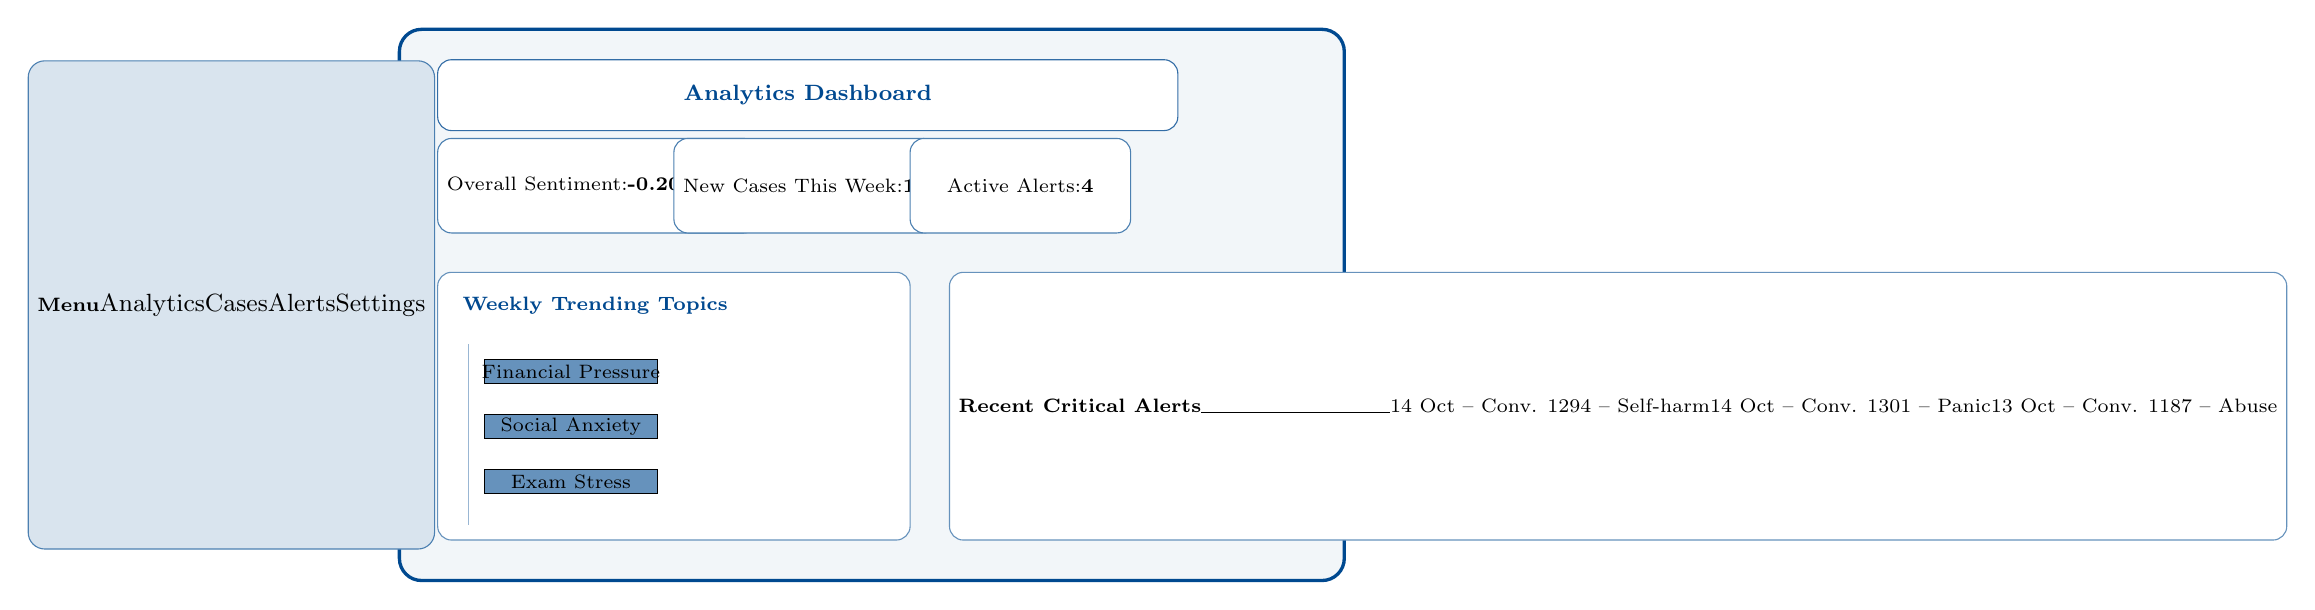
\begin{tikzpicture}[
        screen/.style={rectangle, draw=ugmBlue, very thick, rounded corners=8pt, fill=ugmBlue!5, minimum width=12cm, minimum height=7cm},
        nav/.style={rectangle, draw=ugmBlue!70, fill=ugmBlue!15, align=left, minimum width=1.6cm, minimum height=6.2cm, rounded corners=6pt, font=\scriptsize},
        header/.style={rectangle, draw=ugmBlue!80, fill=white, rounded corners=5pt, minimum width=9.4cm, minimum height=0.9cm, font=\footnotesize\bfseries, text=ugmBlue, align=left},
        card/.style={rectangle, draw=ugmBlue!70, fill=white, rounded corners=5pt, minimum width=2.8cm, minimum height=1.2cm, align=left, font=\scriptsize},
        chart/.style={rectangle, draw=ugmBlue!60, fill=white, rounded corners=5pt, minimum width=6.0cm, minimum height=3.4cm, align=left},
        table/.style={rectangle, draw=ugmBlue!60, fill=white, rounded corners=5pt, minimum width=2.8cm, minimum height=3.4cm, align=left, font=\scriptsize}
    ]
        \node[screen] (frame) {};
        \node[nav, anchor=west] at ([xshift=-4.7cm]frame.west) {\textbf{Menu}\newline\small Analytics\newline Cases\newline Alerts\newline Settings};
        \node[header, anchor=north west] at ([xshift=0.5cm,yshift=-0.4cm]frame.north west) {Analytics Dashboard};

        \node[card, anchor=north west] (kpi1) at ([xshift=0.5cm,yshift=-1.4cm]frame.north west) {Overall Sentiment:\newline\textbf{-0.20} \textcolor{ugmBlue!70}{( 5\,pt)}};
        \node[card, anchor=north west] (kpi2) at ([xshift=3.5cm,yshift=-1.4cm]frame.north west) {New Cases This Week:\newline\textbf{12}};
        \node[card, anchor=north west] (kpi3) at ([xshift=6.5cm,yshift=-1.4cm]frame.north west) {Active Alerts:\newline\textbf{4}};

        \node[chart, anchor=north west] (topicchart) at ([xshift=0.5cm,yshift=-3.1cm]frame.north west) {};
        \node[font=\scriptsize\bfseries, text=ugmBlue, anchor=north west] at ([xshift=0.2cm,yshift=-0.2cm]topicchart.north west) {Weekly Trending Topics};
        \begin{scope}[shift={(topicchart.south west)}]
            \draw[ugmBlue!40, line width=0.6pt] (0.4,0.2) -- (0.4,2.5);
            \foreach \y/\label in {0.6/Exam Stress,1.3/Social Anxiety,2.0/Financial Pressure} {
                \draw[fill=ugmBlue!60] (0.6,\y) rectangle (2.8,\y+0.3);
                \node[font=\scriptsize] at (1.7,\y+0.15) {\label};
            }
        \end{scope}

        \node[table, anchor=north west] (alerttable) at ([xshift=7.0cm,yshift=-3.1cm]frame.north west) {\textbf{Recent Critical Alerts}\newline\rule{2.4cm}{0.2pt}\newline 14 Oct -- Conv. 1294 -- Self-harm\newline 14 Oct -- Conv. 1301 -- Panic\newline 13 Oct -- Conv. 1187 -- Abuse};
    \end{tikzpicture}
    \caption{Admin dashboard main view highlighting KPIs, trending topics, and the most recent critical alerts surfaced by the agents.}
    \label{fig:ui_admin_dashboard}
\end{figure}

\subsubsection{Case Management View}
When a conversation is flagged by the STA, it appears in the case management view, depicted in Figure \ref{fig:ui_case_management}.
\begin{itemize}
    \item \textbf{Design Justification:} To address Dr. Astuti's pain point of being overwhelmed by administrative tasks and her goal of ensuring no student in crisis is missed, this screen is designed for efficiency. It presents a clean, sortable table of all active cases. When a case is selected, it displays the relevant (anonymized) conversation log, the severity level assigned by the STA, and clear action buttons like "Assign to Counselor" or "Mark as Resolved." This streamlines the workflow from automated detection to human intervention.
\end{itemize}

\begin{figure}[h]
    \centering
    \begin{tikzpicture}[
        frame/.style={rectangle, draw=ugmBlue, very thick, rounded corners=8pt, fill=ugmBlue!5, minimum width=12cm, minimum height=6.5cm},
        panel/.style={rectangle, draw=ugmBlue!70, thick, rounded corners=5pt, fill=white, minimum height=5.4cm},
        title/.style={font=\scriptsize\bfseries, text=ugmBlue},
        celltext/.style={font=\scriptsize, align=left}
    ]
        \node[frame] (frame) {};
        \node[panel, minimum width=4.8cm] (list) at ([xshift=-2.1cm]frame.center) {};
        \node[panel, minimum width=6.6cm, right=0.6cm of list] (detail) {};

        \node[title, anchor=north west] at ([xshift=0.2cm,yshift=-0.2cm]list.north west) {Active Cases};
        \node[celltext, anchor=north west] at ([xshift=0.2cm,yshift=-0.7cm]list.north west) {Case ID \hspace{0.3cm} Status \hspace{0.2cm} Severity \hspace{0.2cm} Assigned};
        \foreach \y/\case/\status/\sev/\assignee in {4.4/C-1294/Open/Critical/Dr. Hana,3.6/C-1301/Assigned/High/Dr. Raka,2.8/C-1187/Open/Moderate/--,2.0/C-1150/Closed/Low/Dr. Hana}
            \node[celltext] at ([xshift=0.25cm,yshift=-\y mm]list.north west) {\case\hspace{0.6cm}\status\hspace{0.3cm}\sev\hspace{0.3cm}\assignee};

        \node[title, anchor=north west] at ([xshift=0.3cm,yshift=-0.2cm]detail.north west) {Case C-1294 \textbullet\ Self-harm keywords detected};
        \node[celltext, anchor=north west, align=left] at ([xshift=0.3cm,yshift=-0.8cm]detail.north west) {	extbf{Risk Level:} Critical \quad \textbf{Assigned To:} Pending};
        \node[celltext, anchor=north west, align=left] at ([xshift=0.3cm,yshift=-1.4cm]detail.north west) {	extbf{Chat Excerpt}\newline [Student] ``I feel overwhelmed...''\newline [Aika] ``I'm here with you. Would you like grounding tips?''};
        \node[celltext, anchor=north west, align=left] at ([xshift=0.3cm,yshift=-3.2cm]detail.north west) {	extbf{Counselor Notes}\newline -- schedule immediate outreach\newline -- provide emergency contacts};
        \node[celltext, anchor=south east] at ([xshift=-0.3cm,yshift=0.3cm]detail.south east) {Buttons: Assign \quad Mark Resolved};
    \end{tikzpicture}
    \caption{Case management interface showing the triaged case list alongside the selected conversation context and follow-up actions.}
    \label{fig:ui_case_management}
\end{figure}

\subsection{The User Portal: A Private and Supportive Space}

The User Portal is designed for Budi, the first-year student. The UI prioritizes simplicity, privacy, and a sense of calm, directly addressing his hesitation to seek help and his desire for a non-intimidating support tool.

\subsubsection{The '/aika' Chat Interface}
The core of the student experience is the chat interface, shown in Figure \ref{fig:ui_chat}.
\begin{itemize}
    \item \textbf{Design Justification:} To align with the principle of "Clarity Over Clutter," the interface is intentionally minimalist, resembling modern messaging applications to feel familiar and intuitive. There are no distracting elements; the focus is solely on the conversation between Budi and the Support Coach Agent. This design directly supports his goal of finding a private and focused space to articulate his feelings.
\end{itemize}

\begin{figure}[h]
    \centering
    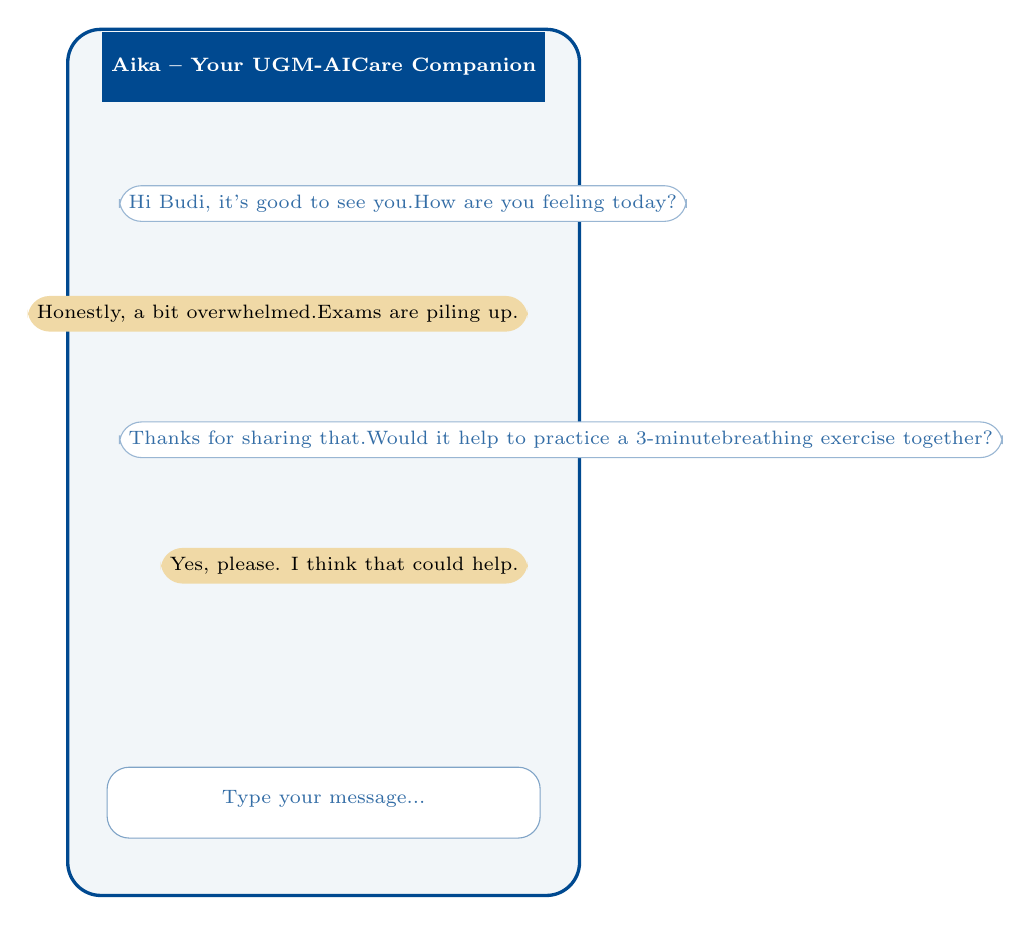
\begin{tikzpicture}[
        phone/.style={rectangle, draw=ugmBlue, very thick, rounded corners=12pt, fill=ugmBlue!5, minimum width=6.5cm, minimum height=11cm},
        header/.style={rectangle, draw=none, rounded corners=0pt, fill=ugmBlue, minimum width=5.5cm, minimum height=0.9cm, font=\scriptsize\bfseries, text=white},
        bubbleUser/.style={rectangle, rounded corners=8pt, fill=ugmGold!40, draw=none, font=\scriptsize, align=left, text=black},
        bubbleAgent/.style={rectangle, rounded corners=8pt, fill=white, draw=ugmBlue!40, font=\scriptsize, align=left, text=ugmBlue!80},
        inputbox/.style={rectangle, draw=ugmBlue!50, rounded corners=8pt, fill=white, minimum width=5.5cm, minimum height=0.9cm}
    ]
        \node[phone] (screen) {};
        \node[header] at ([yshift=-0.5cm]screen.north) {Aika -- Your UGM-AICare Companion};
        \node[bubbleAgent, anchor=north west] at ([xshift=-2.6cm,yshift=-2.0cm]screen.north) {Hi Budi, it's good to see you.\newline How are you feeling today?};
        \node[bubbleUser, anchor=north east] at ([xshift=2.6cm,yshift=-3.4cm]screen.north) {Honestly, a bit overwhelmed.\newline Exams are piling up.};
        \node[bubbleAgent, anchor=north west] at ([xshift=-2.6cm,yshift=-5.0cm]screen.north) {Thanks for sharing that.\newline Would it help to practice a 3-minute\newline breathing exercise together?};
        \node[bubbleUser, anchor=north east] at ([xshift=2.6cm,yshift=-6.6cm]screen.north) {Yes, please. I think that could help.};
        \node[inputbox] at ([yshift=1.2cm]screen.south) {};
        \node[font=\scriptsize, text=ugmBlue!80] at ([yshift=1.25cm]screen.south) {Type your message...};
    \end{tikzpicture}
    \caption{Minimalist chat interface designed to keep the student's attention on the conversation with Aika.}
    \label{fig:ui_chat}
\end{figure}

\subsubsection{The User Dashboard and Progress Tracking}
To foster engagement and a sense of progress, the user dashboard (Figure \ref{fig:ui_user_dashboard}) visualizes the student's journey.
\begin{itemize}
    \item \textbf{Design Justification:} This screen directly supports Budi's goal of feeling a sense of accomplishment. It includes a section for "My Progress" that shows completed modules, highlights recommended next steps, and surfaces gentle reminders for upcoming check-ins. This visual feedback, based on the design principle of "Foster a Sense of Progress," reinforces positive behavior and encourages continued engagement with the platform's coaching features.
\end{itemize}

\begin{figure}[h]
    \centering
    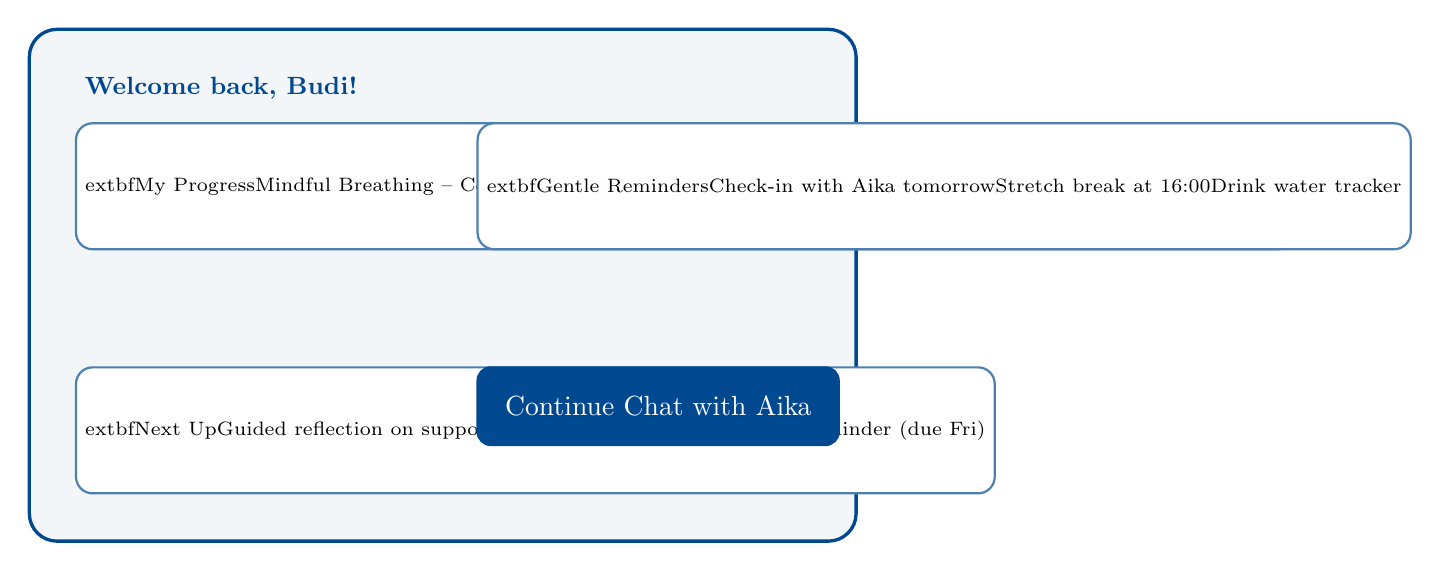
\begin{tikzpicture}[
        card/.style={rectangle, draw=ugmBlue, very thick, rounded corners=10pt, fill=ugmBlue!5, minimum width=10.5cm, minimum height=6.5cm},
        section/.style={rectangle, draw=ugmBlue!70, thick, rounded corners=6pt, fill=white, minimum height=1.6cm, align=left, font=\scriptsize},
        heading/.style={font=\bfseries\small, text=ugmBlue}
    ]
        \node[card] (dash) {};
        \node[heading, anchor=north west] at ([xshift=0.6cm,yshift=-0.5cm]dash.north west) {Welcome back, Budi!};
        \node[section, minimum width=4.6cm, anchor=north west] (progress) at ([xshift=0.6cm,yshift=-1.2cm]dash.north west) {	extbf{My Progress}\newline Mindful Breathing -- Completed 12 Oct\newline Journaling -- Completed 11 Oct\newline Sleep Check-in -- Completed 10 Oct};
        \node[section, minimum width=4.6cm, anchor=north west] (nextup) at ([xshift=0.6cm,yshift=-4.3cm]dash.north west) {	extbf{Next Up}\newline Guided reflection on support network\newline Schedule peer meet-up reminder (due Fri)};
        \node[section, minimum width=4.6cm, anchor=north west] (reminder) at ([xshift=5.7cm,yshift=-1.2cm]dash.north west) {	extbf{Gentle Reminders}\newline Check-in with Aika tomorrow\newline Stretch break at 16:00\newline Drink water tracker};
        \node[rectangle, draw=ugmBlue, rounded corners=5pt, fill=ugmBlue, text=white, minimum width=4.6cm, minimum height=1cm, anchor=north west] at ([xshift=5.7cm,yshift=-4.3cm]dash.north west) {Continue Chat with Aika};
    \end{tikzpicture}
    \caption{Personal dashboard emphasising completed activities, recommended follow-ups, and a clear path back into the coaching conversation.}
    \label{fig:ui_user_dashboard}
\end{figure}

\subsection{Interaction Flows and User Journeys}

While the preceding sections have defined the static components of the user interface, this subsection details the dynamic, step-by-step user journeys for key scenarios. These flows illustrate how a user navigates the application to achieve a specific goal and how the different agents of the Safety Agent Suite collaborate to facilitate these interactions.

\subsubsection{Journey 1: Making an Appointment with a Counselor}
This journey is designed to be as frictionless as possible, directly addressing Budi's hesitation with complex administrative processes.
\begin{enumerate}
    \item \textbf{Initiation:} The user can initiate the process in two ways: either by navigating to an "Appointments" section in the User Portal or by expressing the intent to speak with a counselor during a chat with the Support Coach Agent (SCA).
    \item \textbf{Agent Handoff:} If initiated via chat, the SCA recognizes the intent and calls a tool that invokes the Service Desk Agent (SDA).
    \item \textbf{Scheduling:} The SDA's \texttt{check\_calendar\_availability} tool fetches available time slots from the counselors' calendars and presents them to the user in a simple interface.
    \item \textbf{Confirmation:} The user selects a time slot. The SDA then calls its \texttt{book\_appointment} tool, which confirms the appointment in the system and sends a confirmation notification to both the user and the assigned counselor.
\end{enumerate}

\begin{figure}[h]
    \centering
    \begin{tikzpicture}[
        flowstep/.style={rectangle, rounded corners=4pt, draw=ugmBlue, thick, align=center, fill=ugmBlue!6, minimum width=3.6cm, minimum height=1.1cm, font=\scriptsize},
        flowdecision/.style={diamond, draw=ugmGold!80!black, thick, fill=ugmGold!20, align=center, aspect=2, font=\scriptsize},
        arrow/.style={-Latex, thick, ugmBlue}
    ]
        \node[flowstep] (start) {Student opens booking page\newline or requests help in chat};
        \node[flowdecision, below=1.3cm of start] (viachat) {Initiated via chat?};
        \node[flowstep, below=1.4cm of viachat] (sca) {SCA detects scheduling intent\newline and summarises request};
        \node[flowstep, below=1.2cm of sca] (sda) {SDA checks counselor availability\newline (\texttt{check\_calendar\_availability})};
        \node[flowstep, below=1.2cm of sda] (select) {Student selects preferred slot};
        \node[flowstep, below=1.2cm of select] (confirm) {SDA books appointment\newline (\texttt{book\_appointment})};
        \node[flowstep, below=1.2cm of confirm] (notify) {Confirmations sent to student\newline and assigned counselor};

        \draw[arrow] (start) -- (viachat);
        \draw[arrow] (viachat) -- node[right, font=\scriptsize]{Yes} (sca);
        \draw[arrow] (sca) -- (sda);
        \draw[arrow] (sda) -- (select);
        \draw[arrow] (select) -- (confirm);
        \draw[arrow] (confirm) -- (notify);
        \node[flowstep, right=4.0cm of viachat] (form) {Student fills booking form};
        \draw[arrow] (viachat.east) -- node[above, font=\scriptsize]{No} (form.west);
        \draw[arrow] (form.south) |- (sda.east);
    \end{tikzpicture}
    \caption{Appointment booking journey showing both chat-triggered and self-initiated flows converging on the Service Desk Agent for scheduling and confirmation.}
    \label{fig:journey_appointment}
\end{figure}

\subsubsection{Journey 2: Standard Interaction with Aika (SCA)}
This flow represents the primary use case of the chat interface, where a student seeks supportive conversation.
\begin{enumerate}
    \item \textbf{Initiation:} The user navigates to the `/aika` chat page and sends a message.
    \item \textbf{Real-Time Triage:} The message is first intercepted by the Safety Triage Agent (STA), which performs an instantaneous risk assessment.
    \item \textbf{Safe Handoff:} Assuming the risk is classified as "Low" or "Moderate," the message is passed to the Support Coach Agent (SCA).
    \item \textbf{Conversational Loop:} The SCA generates an empathetic, context-aware response and sends it to the user. This loop (User Message -> STA -> SCA -> User Response) continues for the duration of the conversation.
\end{enumerate}

\subsubsection{Journey 3: Crisis Escalation and Case Management}
This journey illustrates the system's core safety protocol.
\begin{enumerate}
    \item \textbf{Detection:} During a standard conversation, the user sends a message that the STA classifies as "Critical."
    \item \textbf{Automated Escalation:} The STA immediately interrupts the normal flow. It invokes a tool that:
        \begin{itemize}
            \item Displays pre-defined emergency resources to the user.
            \item Sends a high-priority alert to the Admin Dashboard.
            \item Instructs the Service Desk Agent (SDA) to create a new case, linking it to the conversation.
        \end{itemize}
    \item \textbf{Human Intervention:} A counselor (Dr. Astuti) sees the alert on the dashboard, reviews the newly created case, and initiates follow-up. The counselor uses the case management interface to document all actions taken.
\end{enumerate}

\begin{figure}[h]
    \centering
    \fbox{\parbox[c][6cm][c]{0.9\textwidth}{\centering \textbf{Placeholder for Flowchart: Crisis Escalation Journey} \\ \vspace{1cm} This flowchart should show the path from STA detection to the SDA creating a case and the final review by a human counselor on the Admin Dashboard.}}
    \caption{The user and system journey during a critical risk escalation.}
    \label{fig:journey_escalation}
\end{figure}

\subsubsection{Journey 4: Administrator Reviewing Weekly Insights}
This flow describes how an administrator like Dr. Astuti uses the system for strategic planning.
\begin{enumerate}
    \item \textbf{Automated Analysis:} On its pre-defined schedule (e.g., Sunday at midnight), the Insights Agent (IA) is triggered.
    \item \textbf{Report Generation:} The IA queries the anonymized database, performs its analysis, and generates a new strategic report.
    \item \textbf{Notification and Access:} The IA sends an email notification to Dr. Astuti and pushes the new report to the Admin Dashboard.
    \item \textbf{Review:} Dr. Astuti logs into the dashboard, navigates to the analytics view, and reviews the latest trends to inform her weekly planning.
\end{enumerate}

\subsubsection{Journey 5: Proactive Outreach by the SCA}
This journey demonstrates the system's proactive capabilities, closing the loop from insight to intervention.
\begin{enumerate}
    \item \textbf{Configuration:} Based on the IA's report showing a spike in "exam stress," Dr. Astuti configures a proactive outreach campaign from the Admin Dashboard. She targets all active users and selects a pre-defined message offering a time management module.
    \item \textbf{Agent Action:} The system tasks the Support Coach Agent (SCA) to act.
    \item \textbf{User Contact:} The next time a targeted student (Budi) logs into the platform, the SCA initiates the conversation with the configured message, such as, "Hi Budi, with exams coming up, many students are feeling stressed. Would you like to try a quick module on effective study habits?"
\end{enumerate}

\subsubsection{Journey 6: Contextual Module Suggestion}
This flow shows how the SCA provides relevant support within a natural conversation.
\begin{enumerate}
    \item \textbf{Conversation Context:} During a chat, a student (Budi) expresses feelings of anxiety and worry about an upcoming presentation.
    \item \textbf{Intent Recognition:} The SCA, using the reasoning power of the Gemini API, recognizes this as an opportunity to offer a specific, helpful tool.
    \item \textbf{Module Suggestion:} The SCA responds empathetically and then suggests a relevant intervention. For example: "It sounds like that presentation is causing a lot of anxiety. I have a guided breathing exercise that many students find helpful for calming their nerves in moments like this. Would you like to try it?"
    \item \textbf{Module Delivery:} If the user agrees, the SCA invokes its \text{retrieve\_cbt\_module} tool and presents the exercise directly within the chat interface.
\end{enumerate}

%%%%%%%%%%%%%%%%%%%%%%%%%%%%%%%%%%%%%%%%%%%%%%
%%% SECTION 3.8 - SECURITY & PRIVACY %%%
%%%%%%%%%%%%%%%%%%%%%%%%%%%%%%%%%%%%%%%%%%%%%%

\section{Security and Privacy by Design}

Given the profoundly sensitive nature of mental health data, the design and implementation of the UGM-AICare framework are fundamentally guided by the principles of \textbf{Privacy by Design (PbD)}. As established in the theoretical background, PbD dictates that privacy and security must be the default, embedded proactively into the system's architecture from the very beginning, rather than being treated as subsequent additions \cite{FIND_CITATION_PLEASE}. This section details the specific technical and procedural mechanisms implemented to ensure the confidentiality, integrity, and ethical use of user data.

\subsection{Data Anonymization and Minimization}

The cornerstone of the framework's privacy strategy is a multi-layered approach to data anonymization, ensuring that the data used for analytics is irrevocably decoupled from any real-world user identity.

\subsubsection{Application-Layer PII Redaction Pipeline}
To prevent the accidental storage of Personally Identifiable Information (PII), a redaction pipeline is executed within the FastAPI backend for every message received from a user *before* it is written to the \texttt{conversation\_logs} table. This automated process involves:
\begin{enumerate}
    \item \textbf{Pattern Matching:} The system uses regular expressions to identify and remove common PII patterns, such as email addresses, phone numbers, and student ID numbers.
    \item \textbf{Named Entity Recognition (NER):} A lightweight NLP model is used to identify and redact proper nouns that are likely to be names of people or specific locations.
\end{enumerate}
This proactive redaction ensures that the data persisted for long-term storage and analysis is anonymized by default.

\subsubsection{Anonymized User Identifiers}
As detailed in the database design, the system never stores a user's real name, email, or university ID. Each user is assigned a randomly generated Universally Unique Identifier (UUID) upon their first interaction, which serves as their primary key throughout the database. This ensures that even within the system, a user's activity is linked to a pseudonym, not a real identity.

\subsection{Architectural Security Measures}

Beyond anonymization, the framework implements standard, industry-best-practice security measures to protect the integrity and confidentiality of the entire system.

\begin{itemize}
    \item \textbf{Role-Based Access Control (RBAC):} Access to the Admin Dashboard is strictly controlled by an RBAC mechanism. Only authenticated and authorized university staff with an `ADMIN` role may have access to configure the system and view flagged cases.
    \item \textbf{Secure Communication (HTTPS/TLS):} All communication between the user's browser, the Next.js frontend, and the FastAPI backend occurs exclusively over HTTPS, with traffic encrypted using Transport Layer Security (TLS). This prevents eavesdropping and man-in-the-middle attacks, ensuring that all data is confidential while in transit.
    \item \textbf{Data Encryption at Rest:} The PostgreSQL database is configured to encrypt all data at rest. This means that even if an unauthorized party were to gain access to the physical storage on the server, the database files would be unreadable without the encryption keys.
    \item \textbf{Secure Deployment Environment:} The entire application stack is deployed within a secure Virtual Machine provided by PT INA17, protected by firewalls and managed access controls. The Nginx reverse proxy is configured with up-to-date security headers to protect against common web vulnerabilities like cross-site scripting (XSS) and clickjacking.
\end{itemize}

\subsection{Ethical Safeguards and Human Oversight}

Technology alone is insufficient to guarantee ethical operation. Therefore, the system is designed with procedural safeguards that ensure human oversight for all critical functions.

\begin{itemize}
    \item \textbf{Human-in-the-Loop for Safety:} The framework is explicitly designed to be a tool that assists, but does not replace, human counselors. Every critical risk escalation from the Safety Triage Agent (STA) creates a case that requires mandatory review and action by a qualified human professional. The system automates the detection and reporting, but the final clinical judgment and intervention remain firmly in human hands.
    \item \textbf{Purpose Limitation:} The data collected through the chat interface is used for the sole and explicit purposes of providing in-the-moment support, managing clinical escalations, and generating anonymized, aggregated statistics for improving the university's support services. The data is not used for any other purpose, such as academic assessment or disciplinary action. This principle is enforced through the technical separation of the anonymized analytical data from any administrative records.
\end{itemize}

\section{Ethical Considerations and Research Limitations}

The development of an AI-driven framework for mental health support necessitates a thorough examination of the ethical implications and a transparent acknowledgment of the research's limitations. This section addresses these considerations, framing the ethical design choices and defining the boundaries of the study's findings.

\subsection{Ethical Considerations}

The design of the Safety Agent Suite is grounded in the university's fundamental duty of care to its students. The following ethical principles were central to the framework's architecture.

\begin{itemize}
    \item \textbf{Informed Consent and Transparency:} A core ethical requirement is that users must be explicitly informed that they are interacting with an AI system. The user interface must clearly state that "Aika" is an AI assistant and provide a link to a privacy policy that explains in simple terms how their data is anonymized and used for aggregated statistical analysis. Users must provide explicit consent to these terms before beginning their first interaction.
    \item \textbf{The Risk of AI Misinterpretation:} While Large Language Models are powerful, they are not infallible and can misinterpret the nuances of human emotion and language. The most significant ethical risk is the failure to detect a genuine crisis (a false negative). The architecture mitigates this risk through the \textbf{human-in-the-loop} design of the Safety Triage Agent (STA). Every automated escalation is treated as a high-priority alert that requires mandatory review and follow-up by a qualified human counselor, ensuring that the final judgment on safety-critical situations is never left to the machine alone.
    \item \textbf{AI as a Support Tool, Not a Replacement for Therapy:} It is ethically imperative to clearly define the system's role. The UGM-AICare framework is designed as a sub-clinical, supportive tool and a bridge to professional care, not as a substitute for it. The Support Coach Agent (SCA) is programmed to state this boundary clearly and to encourage users to seek professional help for serious or persistent issues, using the Service Desk Agent (SDA) to facilitate the booking process.
    \item \textbf{Data Privacy and Purpose Limitation:} As detailed in the Security and Privacy by Design section, the system is architected to protect user anonymity. Furthermore, the principle of purpose limitation is strictly enforced. The data collected is used only for the explicit purposes of providing in-the-moment support and generating aggregated, anonymized insights to improve the university's services. It is never used for academic assessment, disciplinary action, or any other purpose outside its stated mission.
\end{itemize}

\subsection{Research Limitations}

This study, as a work of Design Science Research focused on the creation and evaluation of a novel artifact, is subject to several important limitations that define the scope of its conclusions.

\begin{itemize}
    \item \textbf{Methodological Limitation: Evaluation of a Prototype:} The evaluation of this framework, as will be detailed in Chapter 4, is based on the functional testing of a proof-of-concept prototype against predefined scenarios. This thesis validates the *technical feasibility* of the agentic workflows and the *architectural integrity* of the design. However, it is not a clinical trial and does not measure the long-term psychological impact or therapeutic efficacy of the system on actual students. Such claims would require a separate, longitudinal study with appropriate clinical oversight.
    \item \textbf{Technical Limitation: Inherent Risks of LLMs:} The framework relies on the Google Gemini 2.5 API. Like all LLMs, it is subject to inherent limitations. These include the potential for the model to reflect biases present in its vast training data and the possibility of generating factually incorrect or nonsensical responses ("hallucinations"). While the system's use of structured tools and prompts is designed to mitigate these risks, they cannot be eliminated entirely.
    \item \textbf{Data Limitation: Use of Simulated Data:} The evaluation of the Insights Agent (IA) will be conducted using anonymized, pre-existing chat logs or simulated data. While this is necessary to protect user privacy during the development phase, it means that the agent's performance has not been validated on the specific linguistic patterns and diversity of a live, campus-wide user base. The effectiveness of the topic modeling and sentiment analysis in a real-world context would require further validation post-deployment.
\end{itemize}








